\chapter{Shower shapes and photon identification}
\label{ch:pid_ss}
\epigraph{\emph{“Champions keep playing until they get it right.”}}{Billie Jean King}

% In \Sect{\ref{subsec:objects:egamma:id}} a very brief description on the identification procedure was described. In the current chapter, a more detailed explanation on the process as well as on the variables used to perform the photon identification is presented. \fixme{elaborate more}

The \ac{ECAL} was presented briefly in \Sect{\ref{subsubsec:atlas:atlas:cals:ecal}}, where the measurement mechanism and all the layers it has were described. In this subdetector, photons deposit their energy via electron-positron pair creation and bremsstrahlung radiation, creating an \ac{EM} shower. The \ac{ECAL} does a great job to compute the energy of the \ac{EM} shower, but identifying the initiating particle remains a challenging task. 
However, by virtue of the different layers and granularities in the \ac{ECAL}, different characteristics of these \ac{EM} showers can be studied, and are encoded by different variables called \acfp{SS}.

This chapter presents all the \acp{SS} that are used to identify real photons from fakes in \Sect{\ref{sec:pid_ss:ss}}. The mentioned variables are heavily used in the process of photon identification, as they provide the separation needed between real and fake photons. For this reason, in \Sect{\ref{sec:pid_ss:pid}}, the optimisation of the photon identification (based on the \acp{SS}) is briefly described, as well as how the photon identification efficiencies are measured in data, using three distinct methods. Finally, \Sect{\ref{sec:pid_ss:ss_differences}} describes one key problematic arising in the simulation of the \acp{SS} and how this is handled, for which a more thorough explanation will be given in the \Ch{\ref{ch:ss_corrections}}.






\section{Shower shapes}
\label{sec:pid_ss:ss}

As mentioned in \Sect{\ref{subsec:objects:egamma:id}}, photon identification relies on rectangular cuts applied to \acp{SS} that lead to an excellent separation power between real isolated photons from fake photons originating from hadrons. These \acp{SSV} are computed from the photon candidates' energy deposits in the \ac{ECAL} and \ac{HCAL} cells, and serve to describe the passage of the photons candidates throughout the calorimeters, characterizing the lateral and longitudinal \ac{EM} showers.

In general, real photons produce narrower energy deposits in the \ac{ECAL}, and have lower leakages to the \ac{HCAL}, compared to those photons proveninent from hadrons, where the presence of additional neighbouring hadrons close to the fake photon tend to widen the showers. Furthermore, since the first layer of the \ac{ECAL} consists on fine strips, it is possible to discriminate photon candidates coming from \(\pizero\to\gamma\gamma\) decays, characterized by two local maxima due to the presence of two nearby photons.

\begin{table}[ht!]
    \caption{Discriminative \acp{SS} used for photon identification. The three columns on the right denote whether the variable is used for the \textit{loose} (L), \textit{medium} (L) or \textit{tight} (T) identification \ac{WP} or not.}
    \centering
    \resizebox{\textwidth}{!}{
        \begin{tabular}{p{.2\textwidth}p{.50\textwidth}p{0.12\textwidth}|p{.01\textwidth}p{.01\textwidth}p{.01\textwidth}}
            \hline
            \hline
            Category  &  Description  &  Name & L & M & T \\
            \hline
            \hline
            Hadronic leakage
            &  Ratio of \et in the first sampling layer of the \ac{HCAL} to \et of the \ac{EM} cluster (used over the ranges \(\abseta<0.8\) and \(\abseta>1.52\))
            &  \(R_{\text{had 1}}\)  & \checkmark & \checkmark & \checkmark\\
            &  Ratio of \et in the \ac{HCAL} to \et of the \ac{EM} cluster (used over the range \(0.8<\abseta<1.37\))
            &  \(R_{\text{had}}\) & \checkmark & \checkmark & \checkmark\\
            \hline
            EM second layer
            &  Ratio of the energy in \(3\times 7\) \(\eta \times \phi\) cells over the energy in \(7 \times 7\) cells centered around the photon cluster position
            &  \(R_{\eta}\) & \checkmark & \checkmark & \checkmark\\
            &  Lateral shower width in \(\eta\) & \(w_{\eta 2}\)  & \checkmark & \checkmark & \checkmark\\
            &  Ratio of the energy in \(3 \times 3\) \(\eta \times \phi\) cells over the energy of \(3 \times 7\) cells centered around the photon cluster position
            &  \(R_{\phi}\) &  & \checkmark & \checkmark\\
            \hline
            EM first layer      
            &  Lateral shower width in 3 strips around the maximum
            &  \(w_{\eta 1}\) or \(w_1\) &  & \checkmark & \checkmark\\
            &  Total lateral width
            &  \(w_{\text{s tot}}\) &  & \checkmark & \checkmark\\
            &  Energy outside the core of the three central cells, within seven cells divided by the energy within the three central strips &  \(f_{\text{side}}\)  &  & \checkmark & \checkmark\\
            &  Difference between the energy associated with the second maximum in the strip layer with the minimum value found between the first and second maxima.
            &  \(\Delta E\)  &  & \checkmark & \checkmark\\
            &  Ratio of the energy difference between the maximum energy deposit and the energy deposit in the secondary maximum in the cluster to the sum of these energies
            &  \(E_{\text{ratio}}\)  &  & \checkmark & \checkmark\\
            &  Ratio of the energy in the first layer to the total energy of the \ac{EM} cluster
            &  \(f_1\) & & \checkmark & \checkmark\\
            \hline
            \hline
        \end{tabular}
    }
    \label{tab:pid_ss:ss:ss_variables}
\end{table}

\begin{figure}[ht!]
    \centering
    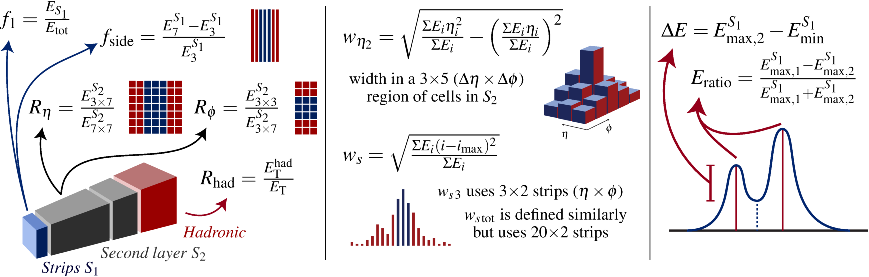
\includegraphics[width=\linewidth]{4_photonid/introduction/diagrams/shower-shapes}
    \caption{Schematic representation of the photon \acp{SS}. The values \(E_C^{S_N}\) represent the energy in layer \(N\) of the \ac{ECAL} in a cluster \(C\).}
    \label{fig:pid_ss:ss:ss_variables}
\end{figure}

In the following, the \acp{SSV} used for photon identification are detailed, shown summarised in \Tab{\ref{tab:pid_ss:ss:ss_variables}} and a scheme of how they are calculated is shown in \Fig{\ref{fig:pid_ss:ss:ss_variables}}.
The first variables make use of the energy measured in the \ac{HCAL}:
\begin{itemize}
    \item Hadronic leakage: is the trasnverse energy deposited in the \ac{HCAL}, normalized to the energy deposited in the \ac{ECAL}:
        \begin{equation}
            {\rhad}_{(1)} = \frac{\et^{\text{had}}}{\et^{\text{EM}}}
        \end{equation}
        In order to minimize the effects of resolution degradation, in the barrel-endcap transition region of the \ac{HCAL} (\(0.8\leq \abseta\leq 1.37\)) the energy deposit in the whole \ac{HCAL} is used (\rhad). On the reminaing of the detector, only the energy deposited in first layer of the \ac{HCAL} is used (\rhado).
\end{itemize}
The following variables use the second-layer information of the \ac{ECAL}:
\begin{itemize}
    \item Lateral energy profile in \(\eta\):
        \begin{equation}
            \reta = \frac{E_{3\times7}^{s2}}{E_{7\times7}^{s2}}
        \end{equation}
        where \(E_{i\times j}^{s2}\) is the energy sum in the second calorimeter layer contained in a window of \(i \times j \) cells (units of \(\eta \times \phi\) cells), centered at the most energetic cell. This variable gives a measure of the showers' width in the \(\eta\) direction.
    \item Lateral energy profile in \(\phi\):
        \begin{equation}
            \rphi = \frac{E_{3\times3}^{s2}}{E_{3\times7}^{s2}}
        \end{equation}
        defined in a similar way as \reta. However, this variable behaves very different for converted and unconverted photons. Due to the action of the magnetic field, the electrons and positrons are curved into opposite directions in \(\phi\), therefore leading to wider \ac{EM} showers for converted photons compared to those from unconverted ones.
    \item Lateral shower width in \(\eta\):
        \begin{equation}
            \weta = \sqrt{
                \frac{\sum E_i \eta_i^2}{\sum E_i}
                -
                \left(\frac{\sum E_i \eta_i}{\sum E_i}\right)^2
            }
        \end{equation}
        measures the proper width of the \ac{EM} shower, where \(E_i\) is the energy in the \(i\)-th cell of the \ac{ECAL}, measured in a window of \(3\times 5 \) cells in \(\eta \times \phi\).
\end{itemize}
The following variables use the information from the first \ac{ECAL} layer, composed of the strip cells that allow for a high \(\eta\) resolution and allows for a good separation between isolated photons from photons product of the \(\pizero\) decay. \Fig{\ref{fig:pid_ss:ss:pizero}} shows the difference in the energy deposited in the \ac{ECAL} between the two cases mentioned previously.
\begin{itemize}
    \item Lateral energy profile in \(\eta\)
        \begin{equation}
            \fside = \frac{E_7^{s1} - E_3^{s1}}{E_3^{s1}}
        \end{equation}
        measures the energy outside the core of the three central strips within a window of 7 cells, divided by the energy in the three central cells.
    \item Lateral shower width in \(\eta\) (3 strips)
        \begin{equation}
            \wone = \sqrt{
                \frac{\sum E_i (i - i_{max})^2}{\sum E_i}
            }
        \end{equation}
        where \(i\) runs over all cells in a window of 3 cells around the highest-energy-cell. This variable measures the width of the \ac{EM} shower in the first layer of the calorimeter.
    \item Lateral shower width in \(\eta\) (full).
        It is defined in a similar way as \wone, but uses all the cells in a window of \(\Delta\eta\times\Delta\phi=0.0625\times 0.2\), corresponding to approximately to \(20\times 2\) strips \(\eta\times\phi\).
    \item Energy difference
        \begin{equation}
            \deltae = E_{\text{max}, 2}^{s1} - E_{\text{min}}^{s1}
        \end{equation}
        represents the energy difference between the second maximum and the minimum reconstructed energy between the two maxima in the strip layer.
    \item Energy ratio
        \begin{equation}
            \eratio = \frac{
                E_{\text{max}, 1}^{s1} - E_{\text{max}, 2}^{s1}
            }{
                E_{\text{max}, 1}^{s1} + E_{\text{max}, 2}^{s1}
            }
        \end{equation}
        is the ratio of energy difference between the two maxima, normalized to the sum of those energies, in the strip layer.
\end{itemize}

\begin{figure}[ht!]
    \centering
    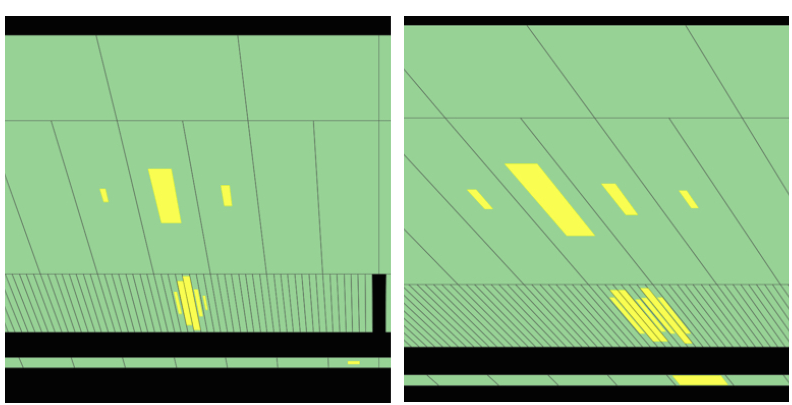
\includegraphics[width=0.7\linewidth]{4_photonid/introduction/diagrams/PhotonPizero}
    \caption{Characteristic energy deposits by an isolated photon (left), and a \(\pizero\to\gamma\gamma\) event (right), which is possible to distinguish thanks to the granularity of the first \ac{ECAL} layer~\cite{ATLAS-ECAL-Pizero}.}
    \label{fig:pid_ss:ss:pizero}
\end{figure}






\section{Photon Identification}
\label{sec:pid_ss:pid}

The identification of prompt photons over fake photons in hadronic collisions is particularly challenging. Fake photons are vastly dominated by reconstructed photon candidates arising from hadron decays in jets, while a smaller fraction of fake candidates are associated with hadrons that deposit significant energy in the \ac{ECAL}, mimicking that of real photons.
Processes with prompt photons in the final state, occurring in \pp collisions at the \ac{LHC}, play a central role in the \ac{ATLAS} physics programme. Either for searches or precision measurements, it is important to rely on excellent algorithms and techniques to identify the real photons over the fake ones. These searches or measurements are performed in a very wide range of the photon \pt, starting from very light Higgs resonances like to a pair of axion-like particles to 4 photons (\(\PH\to aa \to 4\gamma\))~\cite{ATLAS-HiggsTo4Gamma}, where the photon \pt is \(\sim 25~\gev\), up to very high-\pt photons in searches for \gammajet resonances, with photons having \(\pt>1~\tev\). In this section, the procedures for optimising the identification \acp{WP} and measuring the corresponding efficiencies are described.



\subsection{Processes and event selection}
\label{subsec:pid_ss:pid:event_selection}

Given the very wide range in which photons are used in \ac{ATLAS}, the optimisation of the tight identification \ac{WP} relies on two different processes that eventually allow for clean photon samples in the low and high \pt regimes. In the low-\pt case, a very clean source of photons from radiative \Zboson decays are used. On the other hand, although with higher background contamination, \acf{SP} events are employed for high \pt photons. In the following paragraphs, a description of each photon sample is given.


\paragraph{Radiative \Zboson decays}

In the low-\pt range, photons from radiative decays of the \Zboson boson (\(\Zboson \to \ell\ell \gamma\)) are selected as signal photons. There are two different production modes possible for the \ac{SM} \(\pp\to \Zboson(\ellell)\gamma\) processes, where \(\ell\) is either an electron or a moun. These are: \acf{ISR} where the photon is radiated from the quarks, and \acf{FSR} (hereinafter also referred as \acf{RZ} decays), where the photon is radiated from one of the final-state leptons through bremsstrahlung. Both production modes are shown in \Fig{\ref{fig:pid_ss:event_selection:fsr_isr}}.

\begin{figure}[ht!]
    \centering
    \begin{subfigure}[h]{0.49\linewidth}
        \centering
        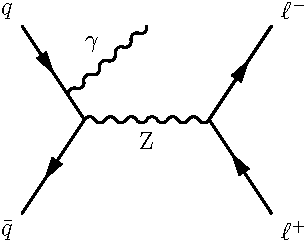
\includegraphics[width=0.6\linewidth]{4_photonid/introduction/diagrams/isr}
        \caption{\acf{ISR}}
    \end{subfigure}
    \hfill
    \begin{subfigure}[h]{0.49\linewidth}
        \centering
        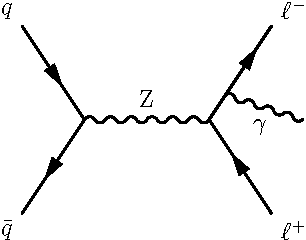
\includegraphics[width=0.6\linewidth]{4_photonid/introduction/diagrams/fsr}
        \caption{\acf{FSR}}
    \end{subfigure}
    \caption{Feynman diagrams for radiative \Zboson decays \(\Zboson\to\ell\ell\gamma\) for the initial-state (left) and final-state (right) radiation.}
    \label{fig:pid_ss:event_selection:fsr_isr}
\end{figure}


Both the \ac{FSR} and \ac{ISR} processes can be easily identified by comparing the two-body invariant mass \mll distribution to the three-body invariant mass \mlly distribution.
For \ac{ISR} events, \mll follows the \Zboson line-shape, and the photon simply adds to the invariant mass making it larger than \(91~\gev\). In the \ac{FSR} case, the three-body invariant mass \mlly follows the \Zboson line-shape, which is seen from \Fig{\ref{fig:pid_ss:event_selection:mll_mlly_distribution:data}}.
For photon identification studies, only photons from \ac{FSR} events are considered. The reason behind the selection of \ac{FSR} over \ac{ISR} is driven by the following. \ac{ISR} events also suffer from \Zjets background contamination, where the jet is misidentified as a photon, and the \Zjets cross-section is magnitudes higher than for \(\Zboson+\gamma\). From \Figs{\ref{fig:pid_ss:event_selection:mll_mlly_distribution:bkg}}{\ref{fig:pid_ss:event_selection:mll_mlly_distribution:signal}}, where the \mll-\mlly distributions are shown for \(\Zboson\to\ell\ell\) and \(\Zboson\to\ell\ell\gamma\) processes, respectively, the separation between these two can be appreciated when selecting \ac{FSR} photons.

With the \ac{RZ} sample, the photons are required to have a transverse momentum \(\pt>7~\gev\) and a pseudorapidity in the range \(\abseta<1.37\) or \(1.52<\abseta<2.37\), to avoid the crack region.
For the optimisation studies no photon isolation is applied, but loose photon isolation, described in \Sect{\ref{subsec:objects:egamma:iso}}, is used for the efficiency measurements. To avoid any biases on the photon footprints in the calorimeter, no other selection is applied for them. Leptons are required to have \(\et>10~\gev\), muons pseudorapidity to be \(\abseta<2.5\) and for electrons \(\abseta<2.47\), excluding the crack. Both electrons and muons need to pass loose isolation requirements and to pass medium identification.

\ac{FSR} photon then are selected by requiring \(80<\mlly<100~\gev\), and \(40<\mll<83~\gev\). Finally, to avoid any biases on the photon \ac{SS} and isolation variables, a minimum distance of \(\DeltaR>0.4\) is required between the photon and the closest lepton.

\begin{figure}[ht!]
    \centering
    \begin{subfigure}[h]{0.32\linewidth}
        \centering
        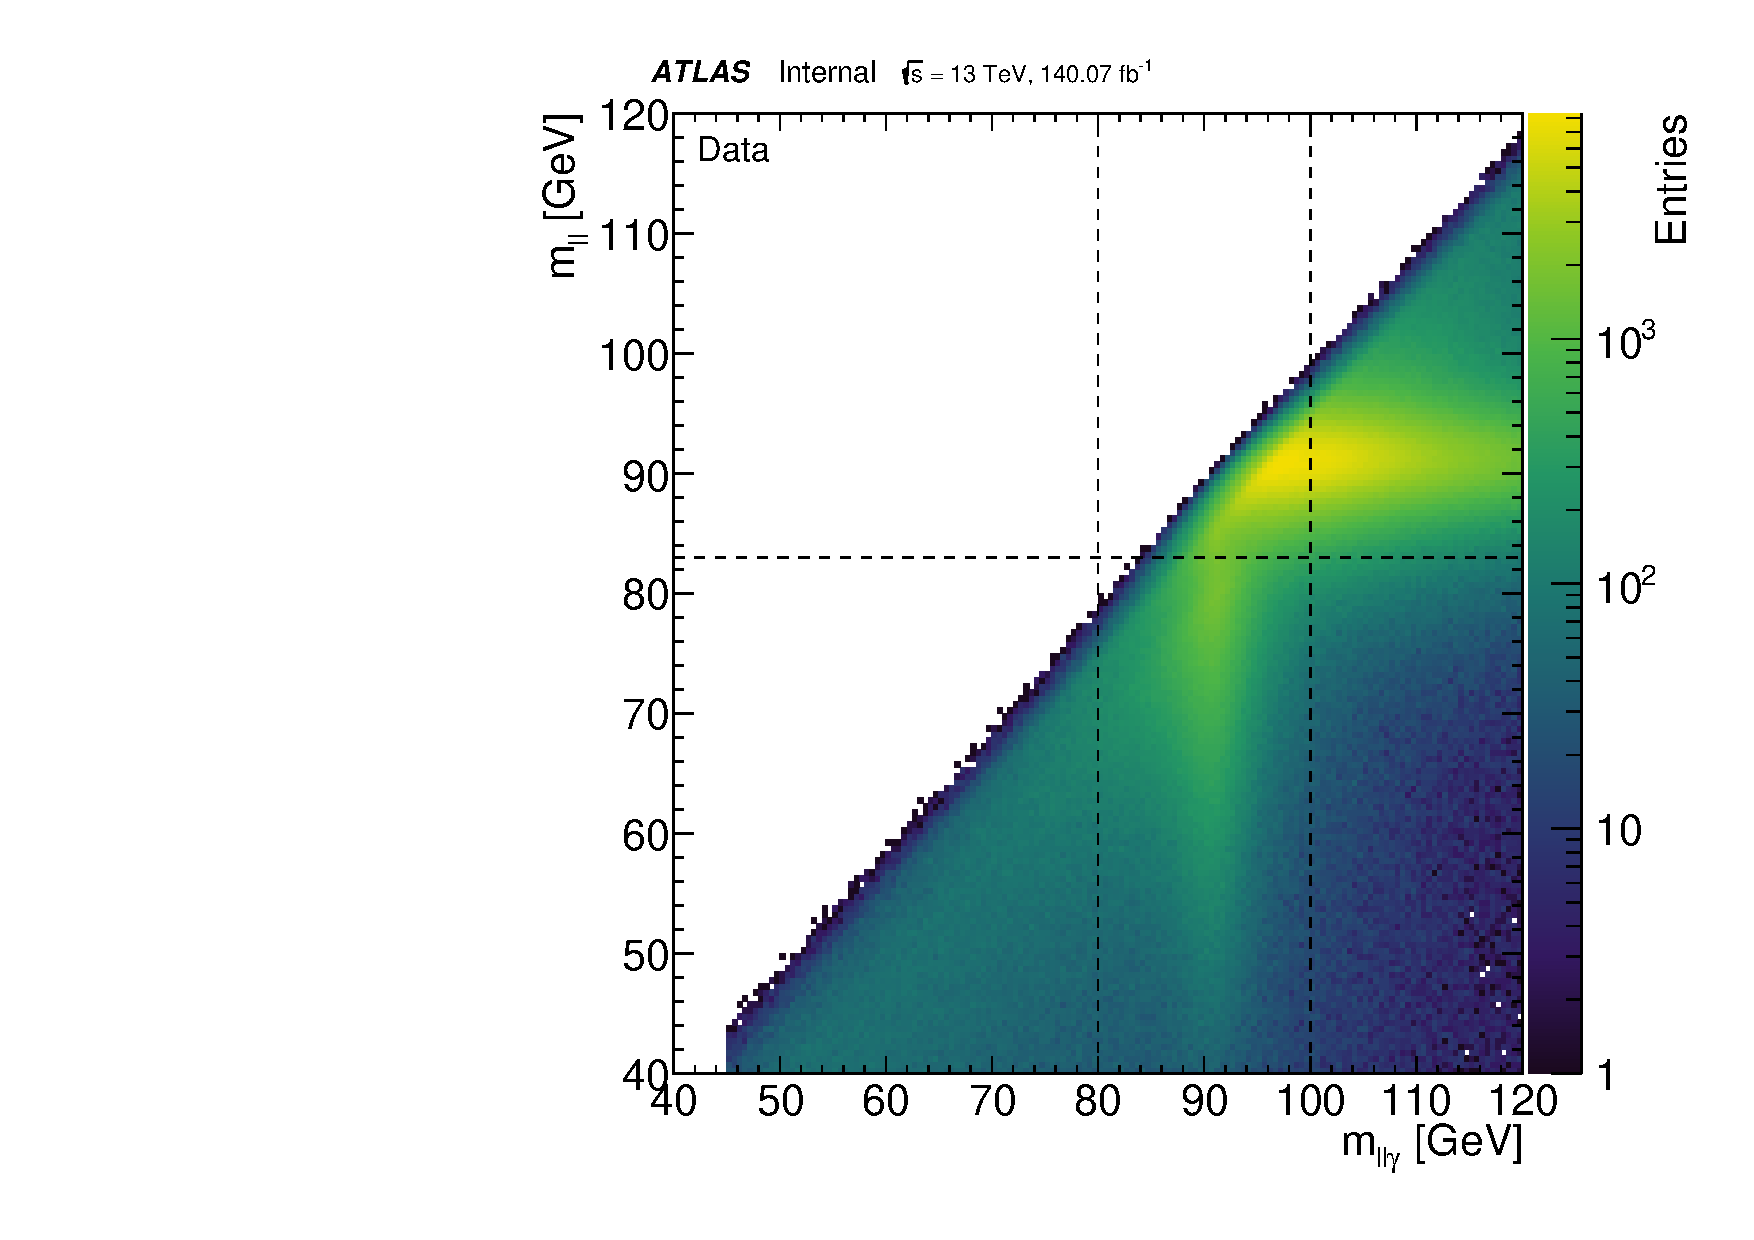
\includegraphics[width=\linewidth]{4_photonid/introduction/can2d__data__nosel__llg_m_ll_m__RZ__rel22_run2_Run2}
        \caption{Data}
        \label{fig:pid_ss:event_selection:mll_mlly_distribution:data}
    \end{subfigure}
    \hfill
    \begin{subfigure}[h]{0.32\linewidth}
        \centering
        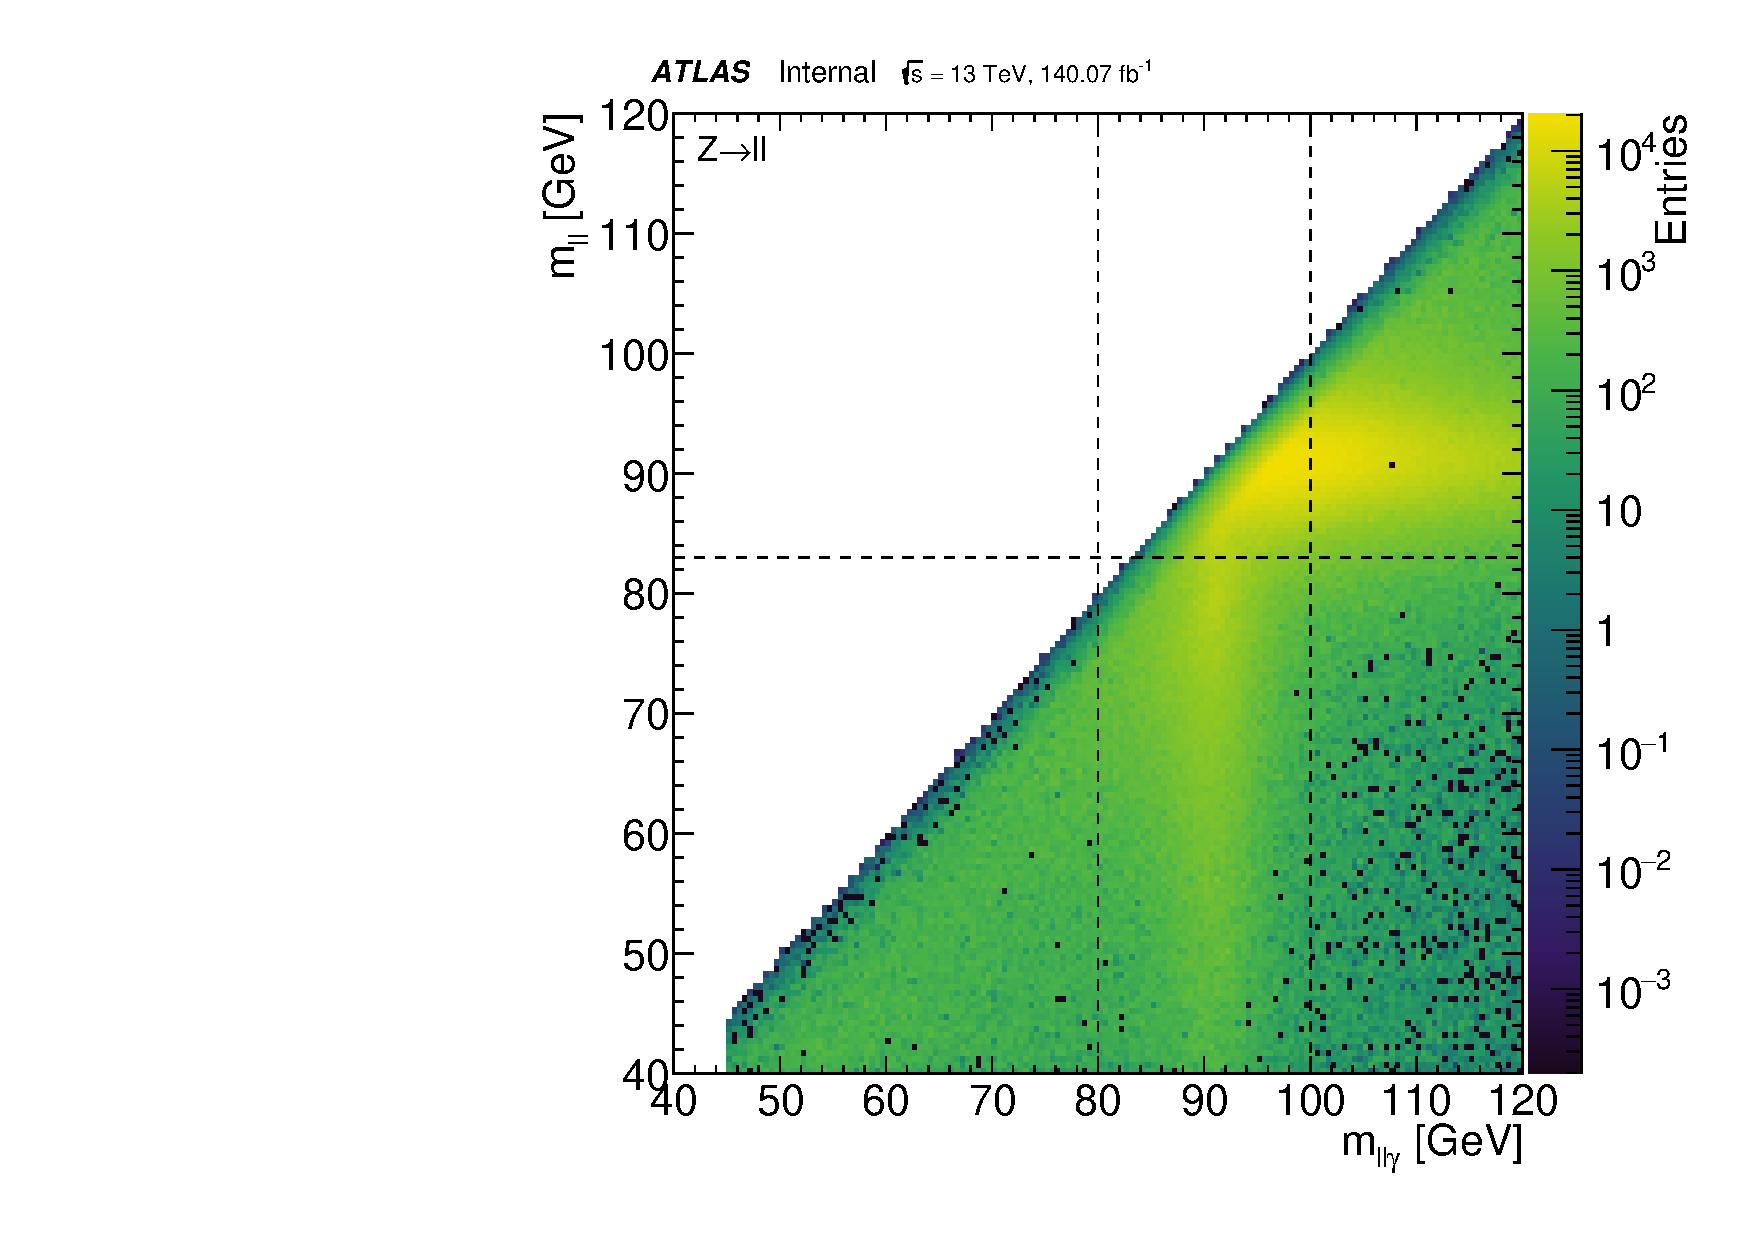
\includegraphics[width=\linewidth]{4_photonid/introduction/can2d__bkg__nosel__llg_m_ll_m__RZ__rel22_run2_Run2}
        \caption{\(\Zboson\to \ell\ell\)}
        \label{fig:pid_ss:event_selection:mll_mlly_distribution:bkg}
    \end{subfigure}
    \hfill
    \begin{subfigure}[h]{0.32\linewidth}
        \centering
        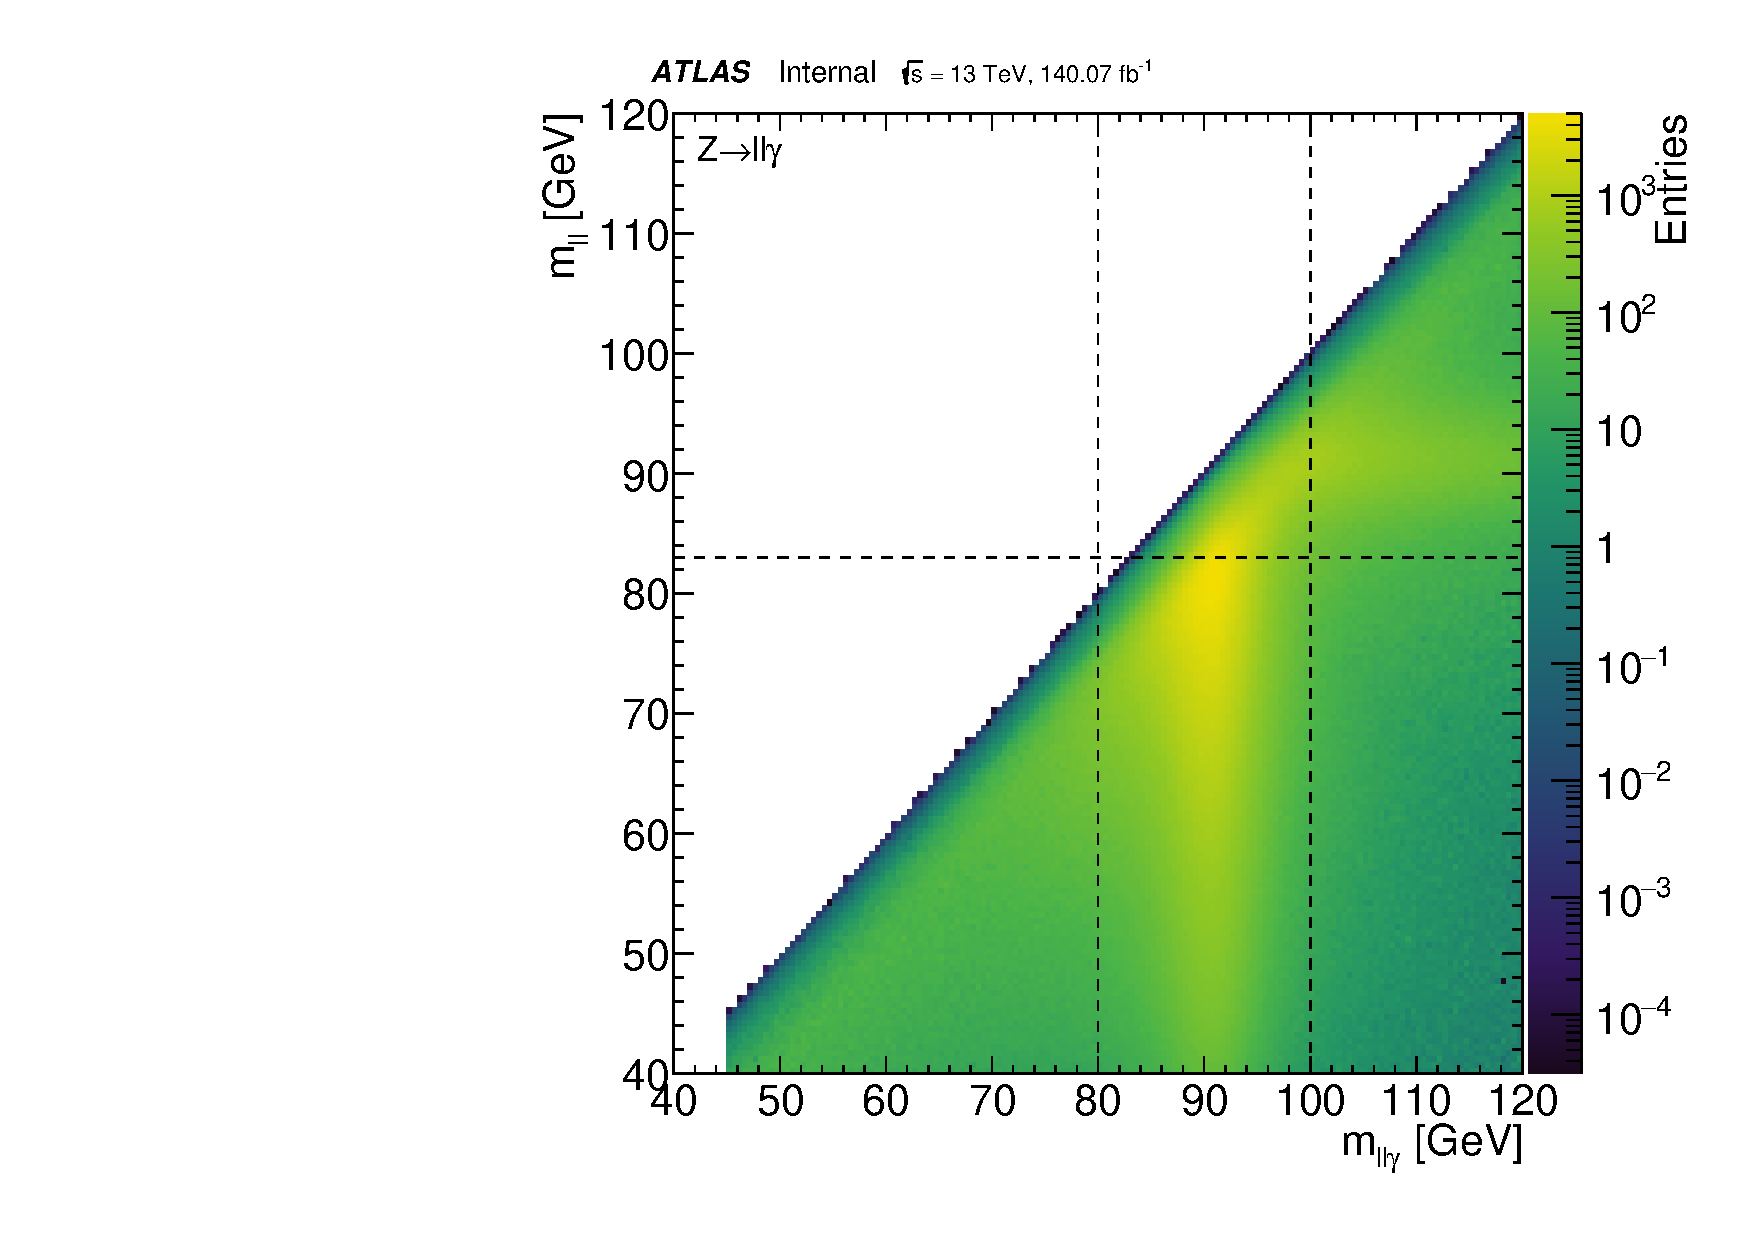
\includegraphics[width=\linewidth]{4_photonid/introduction/can2d__signal__nosel__llg_m_ll_m__RZ__rel22_run2_Run2}
        \caption{\(\Zboson\to \ell\ell\gamma\)}
        \label{fig:pid_ss:event_selection:mll_mlly_distribution:signal}
    \end{subfigure}
    \caption{Two-dimensional invariant mass distribution of the two and three body systems \(m_{\ell\ell}\) and \(m_{\ell\ell\gamma}\), respectively, for (\subref{fig:pid_ss:event_selection:mll_mlly_distribution:data}) data, (\subref{fig:pid_ss:event_selection:mll_mlly_distribution:bkg}) background and (\subref{fig:pid_ss:event_selection:mll_mlly_distribution:signal}) signal. The region in which there is a high concentration of events for \(m_{\ell\ell} \sim m_{\Zboson}\) corresponds to \ac{ISR} events, while \ac{FSR} events can be identified when \(m_{\ell\ell\gamma} \sim m_{\Zboson}\).}
    \label{fig:pid_ss:event_selection:mll_mlly_distribution}
\end{figure}

\paragraph{\acf{SP}}

The inclusive photon, or \acf{SP} sample is collected by single-photon triggers, whose thresholds range from \(10~\gev\) up to \(140~\gev\) and require loose photon identification. Although the triggers used to obtain this sample are prescaled (with the exception of the \(140~\gev\) one) the provide very large photon datasets for high \pt.
These processes include leading-order \gammajet events from \(qg\to q\gamma\) and \(\qqbar \to g\gamma\) hard scattering, as well as prompt photons from quark fragmentation in \ac{QCD} dijet events.
Photons from these events are required to satisfy \(\abseta<2.37\) excluding the crack, and to pass the loose isolation requirement. The \ac{SP} samples are used for both the optimisation and measurements studies.


\subsection{Optimisation}
\label{subsec:pid_ss:pid:optimisation}

Starting from these discriminating \acp{SS}, three \acp{WP} can be defined for photons: \textit{loose}, \textit{medium} and \textit{tight}~\cite{ATLAS-EGamma-Performance-2024}. The loose \ac{WP} employs cuts to the variables defined in the second layer and to the hadronic leakage variable, used primarily by the trigger.
The medium and tight \acp{WP} use all the previsouly defined variables. The former is optimised to have a flat \(95\%\) efficiency, while the latter provides an excellent background rejection. \Tab{\ref{tab:pid_ss:ss:ss_variables}} shows which variables are used for each \ac{WP}.

The optimisation of the \acp{WP} uses two different samples: \ac{RZ} events for photons with \(10<\pt<25~\gev\) as signals and \(\Zboson\to \ell\ell\) as backgrounds; and for the high-\pt regime (\(\pt>25~\gev\)) \ac{SP} events are considered signals while dijet events are the backgrounds.

As previously mentioned, photon identification uses cuts to photon \acfp{SS}. Examples of the \reta, \eratio and \weta \ac{SS} comparing signal and background events using the \ac{RZ} samples are shown in \Fig{\ref{fig:pid_ss:optimisation:shower_shapes}}, where excellent discriminating power is seen.
The cuts on all the \acp{SS}, for each identification \ac{WP}, are optimised as a function of the transverse energy and the pseudo-rapidity of the photon candidate, to account for the shape of the variables for different \(\eta\) and for variations in the amount of material and the geometry of the calorimeter. The medium and tight \acp{WP} are also optimised separately for converted and unconverted photons.
The cuts are optimised using a \ac{MV} approach, where signal efficiencies are scanned between \(0\%\) and \(100\%\) while trying to maximise the background rejection. The resulting, optimised, cut values are subject to fluctuations and therefore they are manually smoothed.

\begin{figure}[ht!]
    \centering
    \begin{subfigure}[h]{0.32\linewidth}
        \centering
        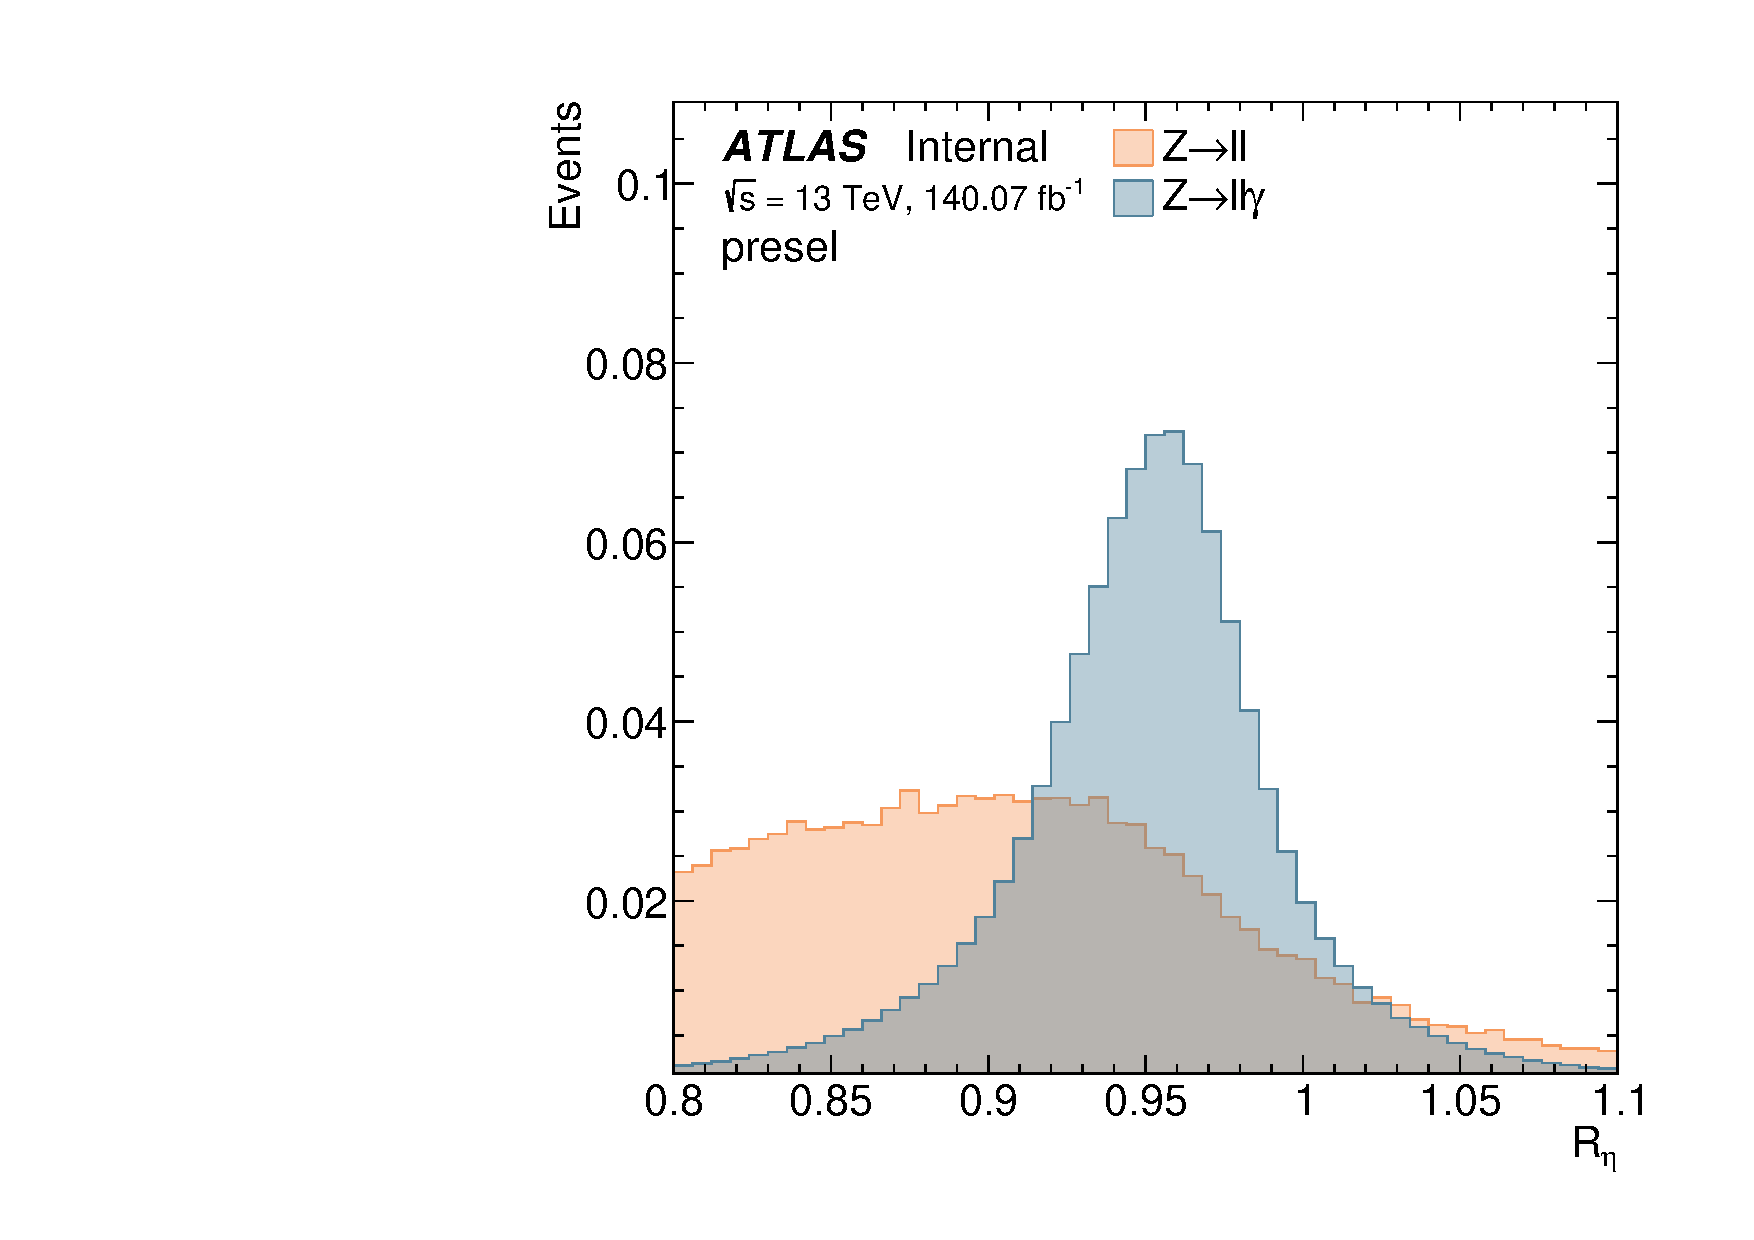
\includegraphics[width=\linewidth]{4_photonid/introduction/shower_shapes/can__sigbkg__presel__ph_reta__RZ__rel22_run2_Run2}
        \caption{\reta}
        \label{fig:pid_ss:optimisation:shower_shapes:reta}
    \end{subfigure}
    \hfill
    \begin{subfigure}[h]{0.32\linewidth}
        \centering
        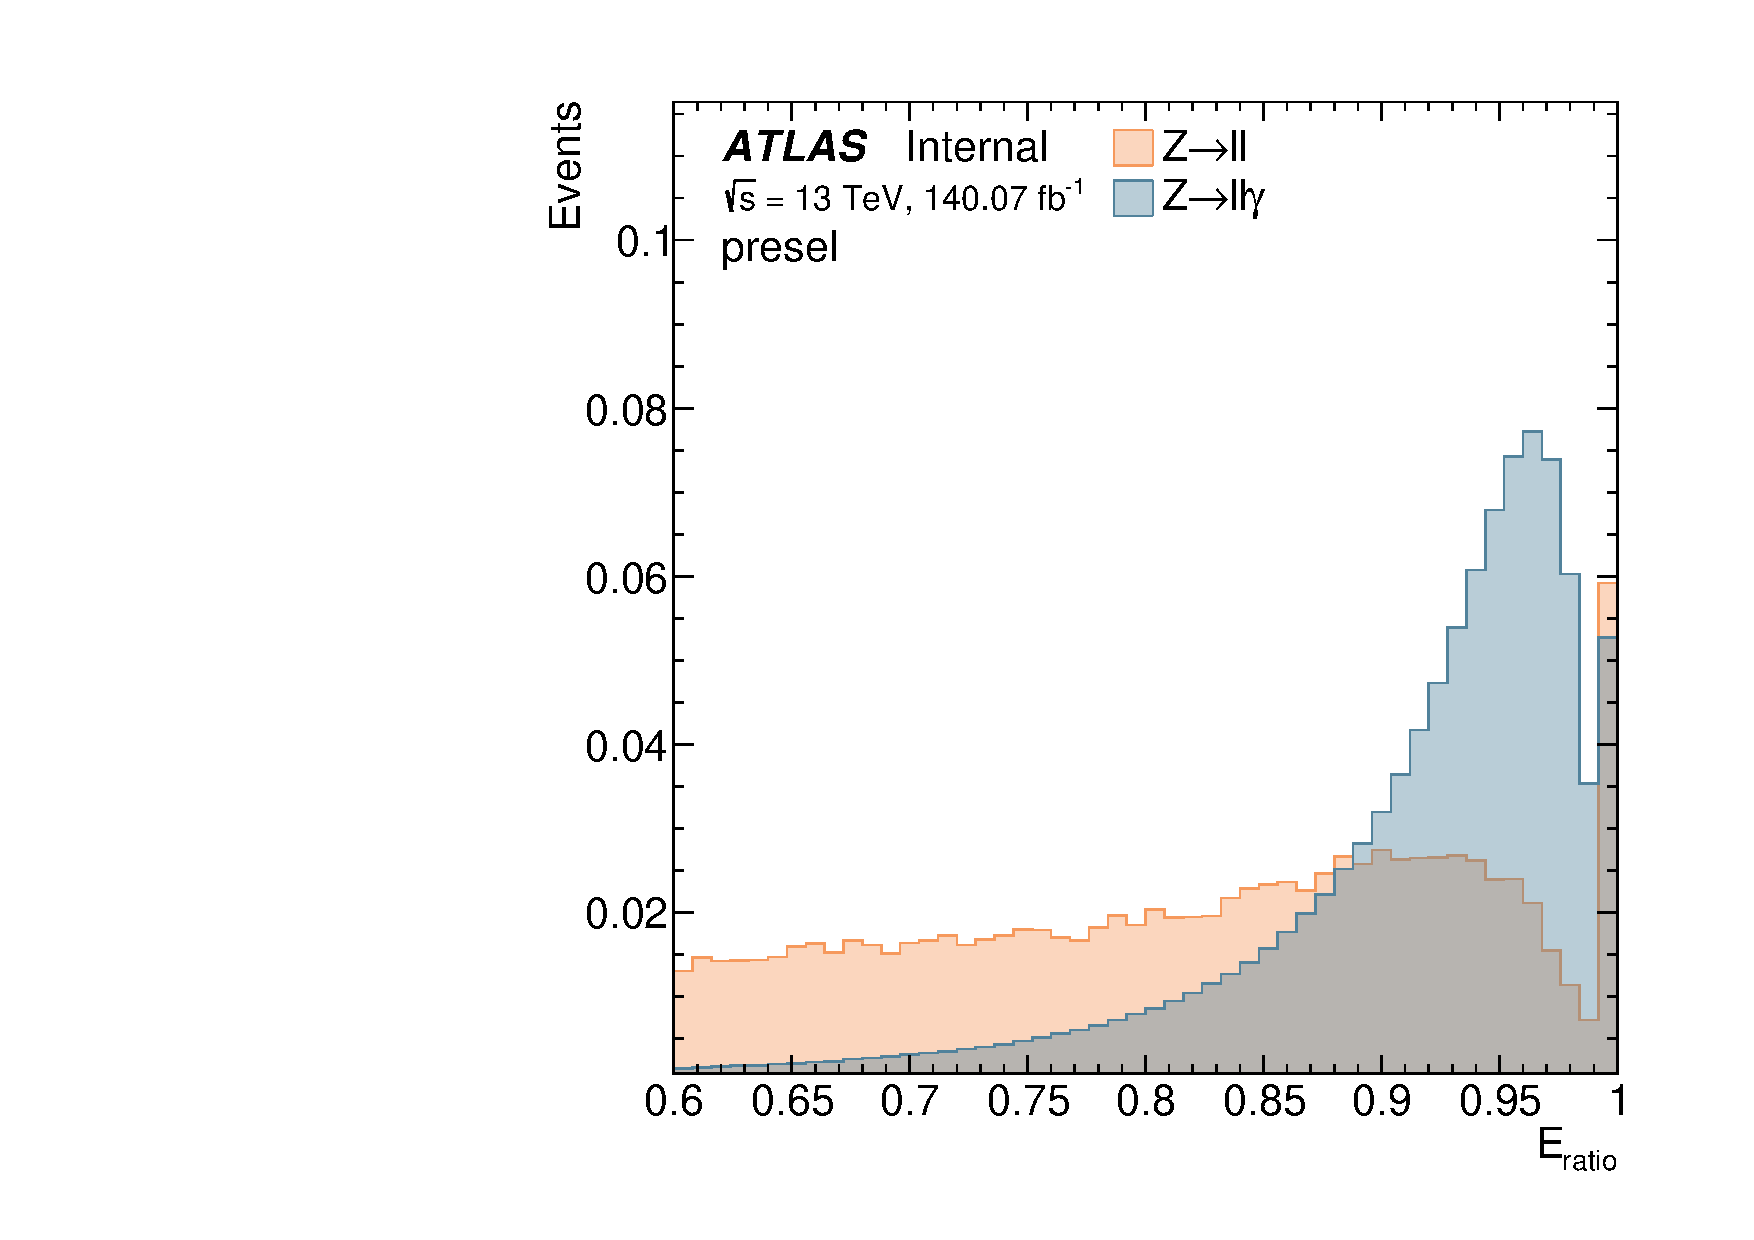
\includegraphics[width=\linewidth]{4_photonid/introduction/shower_shapes/can__sigbkg__presel__ph_eratio__RZ__rel22_run2_Run2}
        \caption{\eratio}
        \label{fig:pid_ss:optimisation:shower_shapes:eratio}
    \end{subfigure}
    \hfill
    \begin{subfigure}[h]{0.32\linewidth}
        \centering
        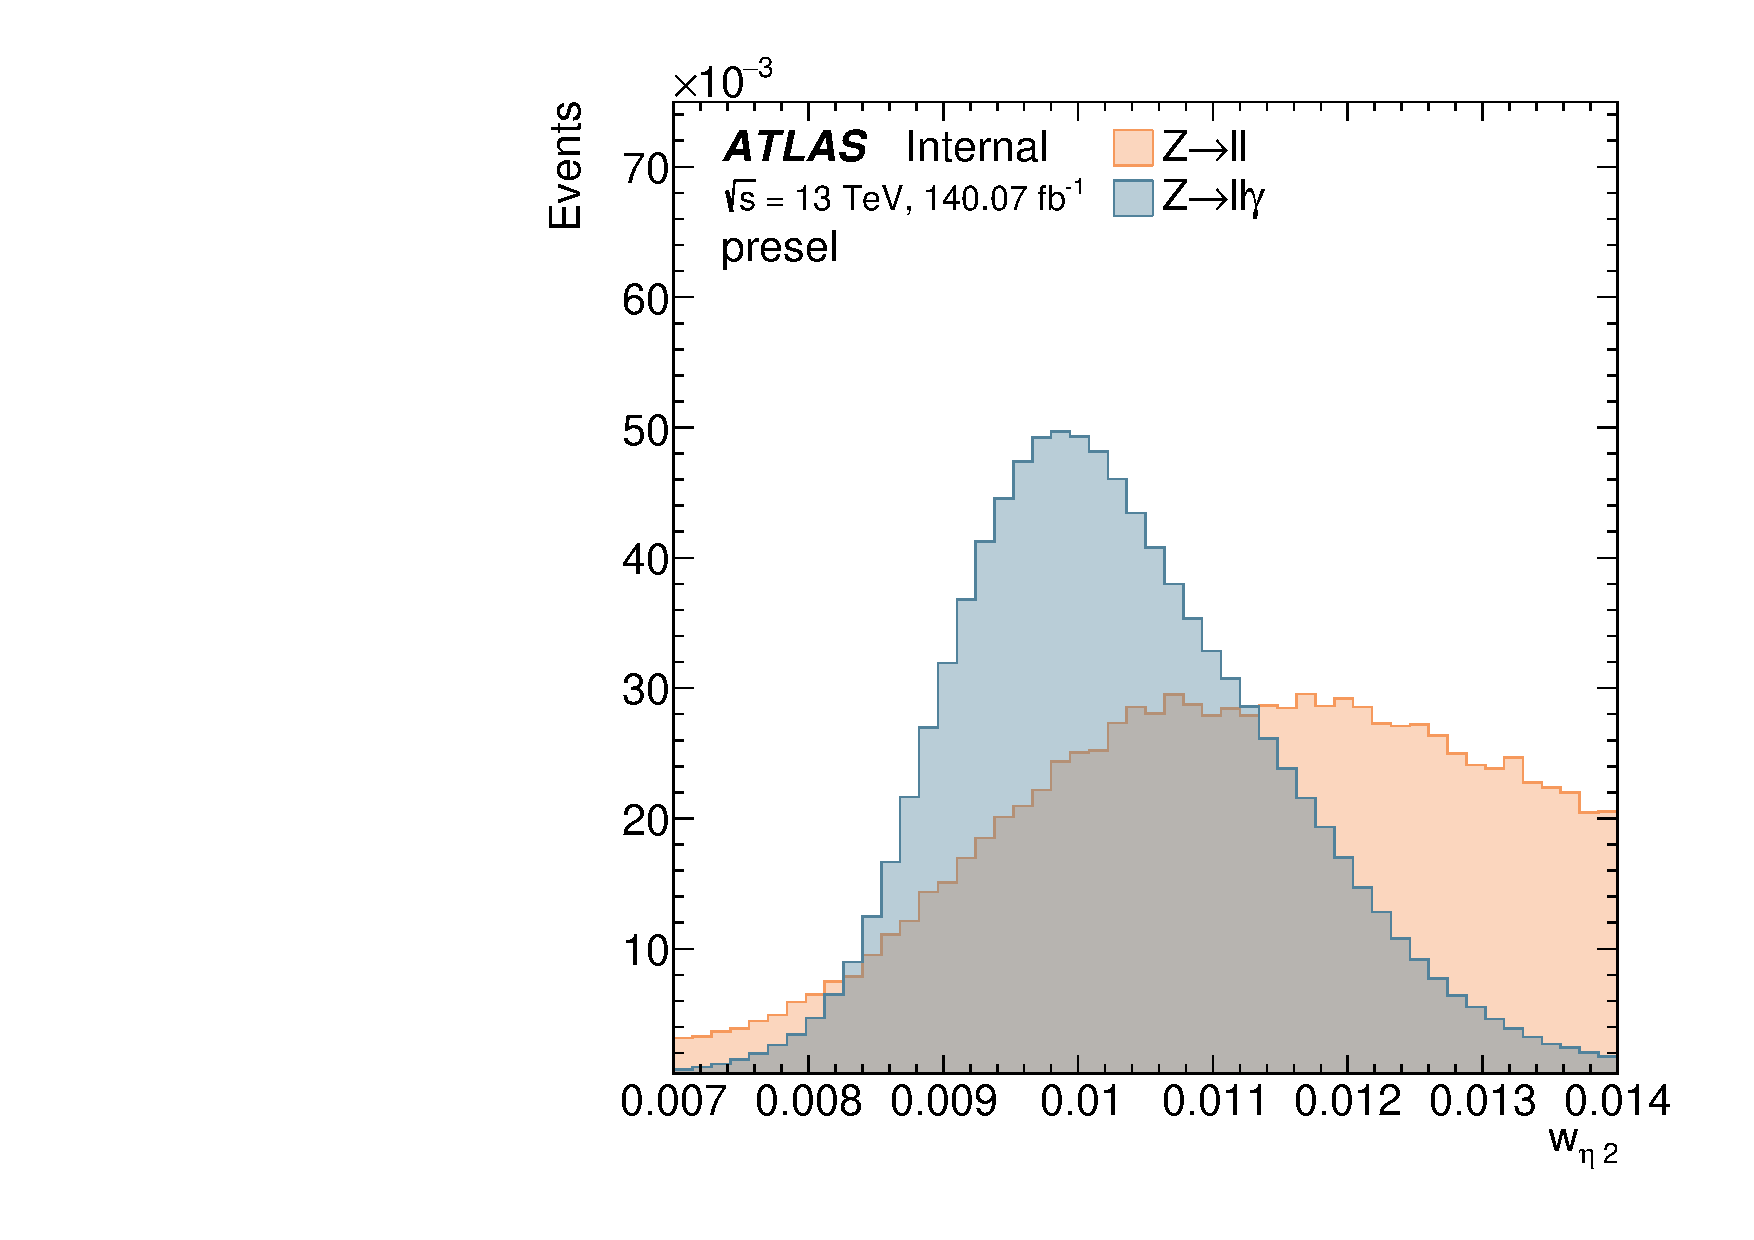
\includegraphics[width=\linewidth]{4_photonid/introduction/shower_shapes/can__sigbkg__presel__ph_weta2__RZ__rel22_run2_Run2}
        \caption{\weta}
        \label{fig:pid_ss:optimisation:shower_shapes:weta2}
    \end{subfigure}
    \caption{Normalised signal (blue) and background (orange) distributions for different \acp{SS}, using \ac{RZ} event samples, passing the event selection detailed in \Sect{\ref{subsec:pid_ss:pid:event_selection}}.}
    \label{fig:pid_ss:optimisation:shower_shapes}
\end{figure}



\subsection{Efficiency measurements}

The maost used \ac{WP} for precision measurements and general searches in \ac{ATLAS} is the tight \ac{WP}. Once the cuts to the \acp{SS} are optimised as previously explained, data and \ac{MC} identification efficiencies are calculated. In all cases, photons are required to satisfy the loose isolation criterion defined in \Sect{\ref{subsec:objects:egamma:iso}} and therefore the photon efficiencies are measured relative to this isolation criterion. These measurements are carried out using three different methods that are detailed in \Refn{\cite{ATLAS-EGamma-Performance-2015-2016}} and in the following paragraphs, a brief description of each method is given.

For the lower \pt range (\(7<\pt<100~\gev\)), photons from radiative \Zboson decays are used as signal photons.
The process to estimate the efficiencies relies on using template fits to the observed three-body invariant-mass (\mlly) distribution before and after applying the tight identification criteria. The number of signal and background events can then be counted from the fits, and signal purities are computed each time: \(P^{\text{total}}\) before applying tight identification and \(P^{\text{pass}}\) after.
The final efficiency in data is then given by
\begin{equation}
    \varepsilon_{ID} = \frac{ P^{\text{pass}} N_{\text{data}}^{\text{pass}} }{ P^{\text{total}} N_{\text{data}}^{\text{total}} }.
\end{equation}

The second method to compute efficiencies relies on Smirnov transformations~\cite{SmirnovTransform} to the electrons' \acp{SS} to resemble those of photons'. The samples used in this approach are \(\Zboson\to ee\) decays, in which the electrons are required to pass loose photon isolation. The candidate electrons in data contain a small background from \Wjets and multijet production; this background is subtracted by fitting simulated signal samples and background templates derived from data control regions to the \(m_{ee}\) data distributions. The electron candidates are counted from events in the range \(70 < m_{ee} < 110~\gev\), and the efficiencies are measured using the tag-and-probe method described in \Refn{\cite{ATLAS-EGamma-Performance-2015-2017}}. The \pt range in which this method is implemented is \(25<\pt<250~\gev\).

The final and third method uses \ac{SP} samples with photons in the range \(50<\pt<1500~\gev\). The matrix method~\cite{ATLAS-EGamma-Performance-2015-2016} is used in this case, which constructs four orthogonal regions that either pass or fail the tight identification \ac{WP}, and pass or fail track-isolation (described in \Sect{\ref{subsec:objects:egamma:iso}}). For each region, two unknowns arise: the number of signal and background events.
If the track isolation efficiencies are known for the signal and background components, then it is possible to estimate the efficiency for loose photons passing the tight identification criteria. The isolation efficiencies for signal photons are estimated using \ac{MC} samples, and the ones for backgrounds are obtained in a jet-enriched control region constructed by inverting the identification criteria.
The efficiency measurements in data for the tight identification \ac{WP} then reads:
\begin{equation}
    \varepsilon^{\text{tight-ID}} = \frac{
        \frac{
            \hat{\varepsilon}_{\text{ID}} - \hat{\varepsilon}_{\text{ID}}^b
        }{
            \hat{\varepsilon}_{\text{ID}}^s - \hat{\varepsilon}_{\text{ID}}^b
        }
        \cdot
        N_{\text{ID}}^T
    }{
        \frac{
            \hat{\varepsilon} - \hat{\varepsilon}^b
        }{
            \hat{\varepsilon}^s - \hat{\varepsilon}^b
        }
        \cdot
        N^T
    },
\end{equation}
where \(N^T\) accounts for the totality of photons in the inclusive sample which consists on \(N^s\) prompt photons (or signal photons) and \(N^b\) fake photons (background photons). The number \(N^T_{\text{ID}}\) is the subset of \(N^T\) that pass the identification requirement. Data, signal and background track isolation efficiencies are represented by \(\hat{\varepsilon}\), \(\hat{\varepsilon}^s\) and \(\hat{\varepsilon}^b\), respectively. Similarly, the track isolation efficiencies for those photons passing tight identification are shown as \(\hat{\varepsilon}_{\text{ID}}\), \(\hat{\varepsilon}_{\text{ID}}^s\) and \(\hat{\varepsilon}_{\text{ID}}^b\), respectively. The measured efficiencies for photons with \(\pt>150~\gev\) is between \(90\) and \(96\%\).





\begin{figure}[ht!]
    \centering
    \begin{subfigure}[h]{0.49\linewidth}
        \centering
        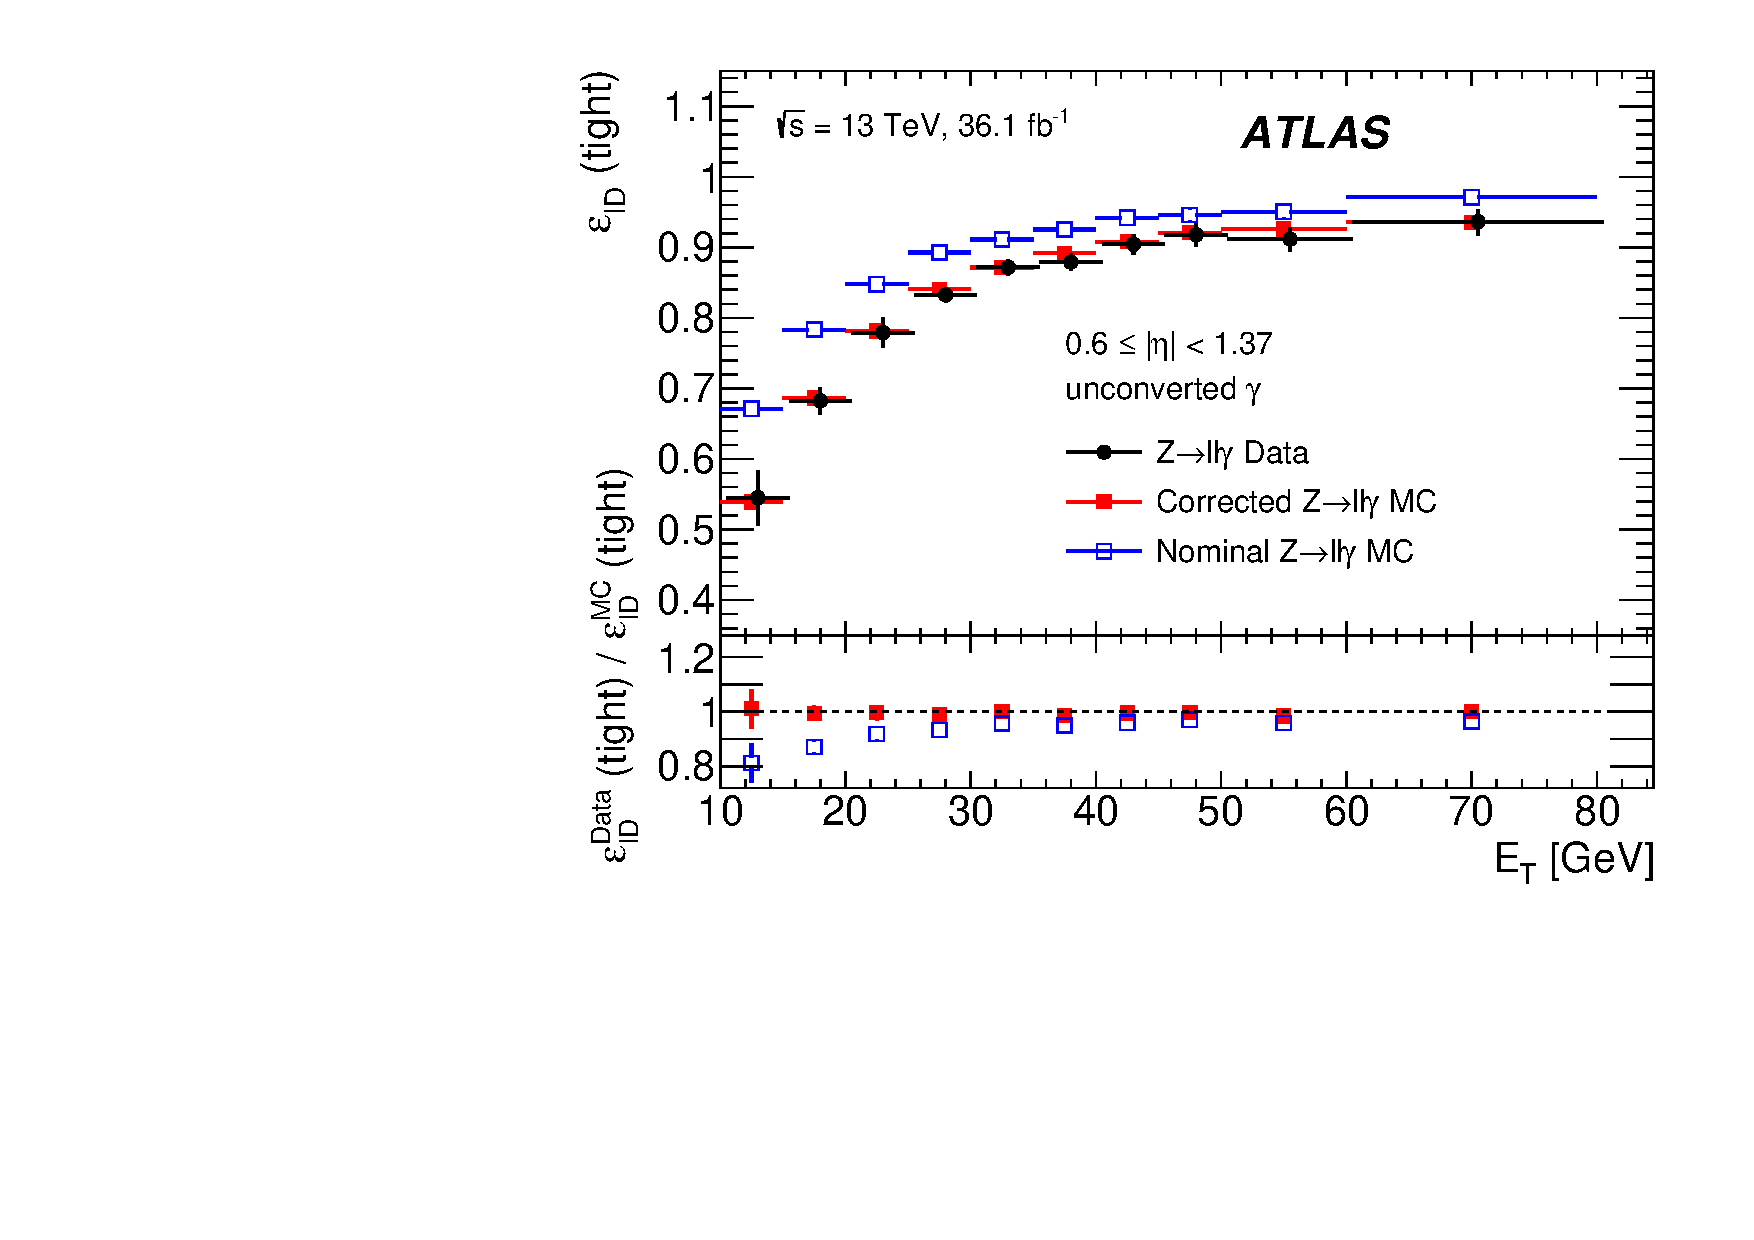
\includegraphics[width=\linewidth]{4_photonid/introduction/efficiencies/pid_rz_efficiency_corrections_comparison}
        \caption{\acf{RZ} method}
        \label{fig:pid_ss:pid:efficiencies:efficiencies_old:rz}
    \end{subfigure}
    \hfill
    \begin{subfigure}[h]{0.49\linewidth}
        \centering
        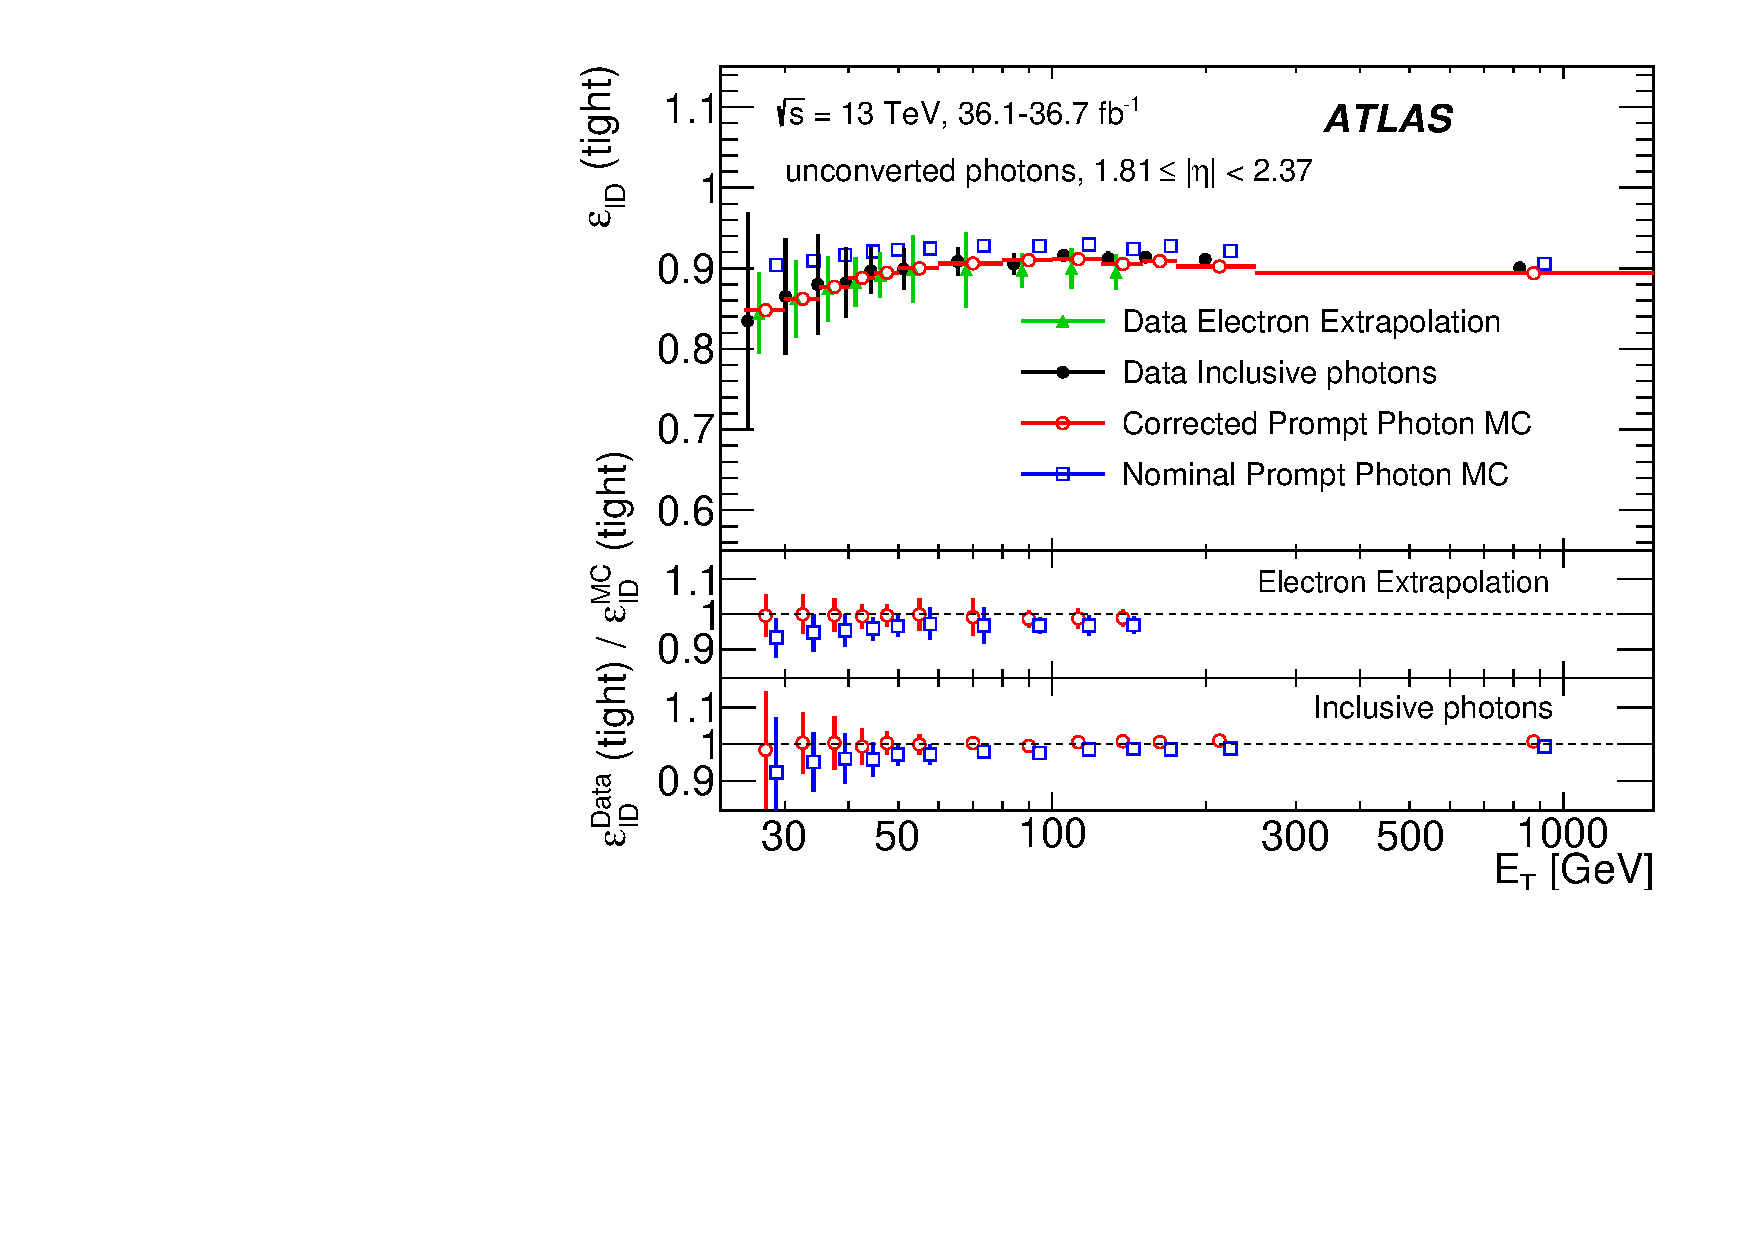
\includegraphics[width=\linewidth]{4_photonid/introduction/efficiencies/pid_ee_sp_efficiency_corrections_comparison}
        \caption{Electron-extrapolation and Matrix-Method}
        \label{fig:pid_ss:pid:efficiencies:efficiencies_old:ee_sp}
    \end{subfigure}
    \caption{Comparison of the measurements between data and \ac{MC} of the three distinct data-driven methods to compute efficiencies. In both figures, for each method, two different set of \ac{MC} measurements are displayed: the nominal one and the corrected one. The bottom panels show the ratio of data efficiencies to \ac{MC} predictions (referred as \acfp{SF} in the text). The figures are taken from \Refn{\cite{ATLAS-EGamma-Performance-2015-2016}}.}
    \label{fig:pid_ss:pid:efficiencies:efficiencies_old}
\end{figure}


Example of the photon identification efficiencies as a function of the photon \pt using the \ac{RZ} method is shown in \Fig{\ref{fig:pid_ss:pid:efficiencies:efficiencies_old:rz}}. Data efficiencies are represented by the black points, while nominal \ac{MC} is shown with blue empty squares. The ratios of data to \ac{MC} (also referred as \acfp{SF}) shown in the bottom pad using the nominal \ac{MC} vary up to 20\%, showing that the simulation is not correctly describing the data. However, another set of \ac{MC} efficiencies is displayed, in this case using corrected \ac{MC}, which drastically improves the agreement between data and simulation, as seen from the \acp{SF}. The reason why these corrections are needed and how they were implemented in \ac{ATLAS} is explained in the following section (\Sect{\ref{sec:pid_ss:ss_differences}}), and how they are currently corrected in \Ch{\ref{ch:ss_corrections}}. \Fig{\ref{fig:pid_ss:pid:efficiencies:efficiencies_old:ee_sp}} shows the efficiency measurements using the two remaining methods (electron-extrapolation and matrix-method), where the same improvements on the \acp{SF} is obtained when using the corrected \ac{MC} simulation.

As mentioned above, these ratios between data and \ac{MC} efficiencies are referred as \acfp{SF} and they encapsulate the differences between data and simulation. They are computed separately for each one of the three methods and are later combined using a weighted average~\cite{BLUEMethod} in each bin and assuming the statistical and systematic uncertinaties to be uncorrelated between the methods. Current results of these \acp{SF}, computed using the full Run-2 dataset, are shown in \Fig{\ref{fig:pid_ss:pid:efficiencies:sfs}}.

\begin{figure}[ht!]
    \centering
    \begin{subfigure}[h]{0.49\linewidth}
        \centering
        \includegraphics[width=\linewidth]{example-image}
        \caption{Converted photons.}
    \end{subfigure}
    \hfill
    \begin{subfigure}[h]{0.49\linewidth}
        \centering
        \includegraphics[width=\linewidth]{example-image}
        \caption{Unconverted photons.}
    \end{subfigure}
    \caption{Photon identification \acp{SF} in the different \pt-\abseta bins for both converted (left) and unconverted photons (right). \fixme{Ask fran for the plots in his presentation!}}
    \label{fig:pid_ss:pid:efficiencies:sfs}
\end{figure}


\section{Shower shapes variables differences between data and MC}
\label{sec:pid_ss:ss_differences}


The \ac{ATLAS} \ac{MC} simulation does not perfectly describes data. This is clearly seen when computing the previsously mentioned \acp{SF}, whose values were different from 1, meaning that different efficiencies are obtained between data and in \ac{MC}. In particular, when comparing the \acp{SS} distributions, it is seen that \ac{MC} distributions are shifted or even the whole shape differs, as shown in \Fig{\ref{fig:pid_ss:ss_differences:ss}}, by comparing data (black dots) against the red line histogram corresponding to \ac{MC}.

The main differences on the distributions arise for the \(\eta\) shower profiles, where broader distributions are seen in data compared to \ac{MC}. Part of the effect was corrected in 2010 after moving to detailed description of the material composition in the accordion absorbers in \textsc{Geant4}. However, the remaining data-\ac{MC} disagreements are still under study and could be due to several potential effects:
\begin{itemize}
    \item Detector geometry description of the lead thickness (including possible variations due to gravity).
    \item Mismodeling of the electric field in the \ac{LAr} gaps.
    \item Mismodeling of the cross-talk effect (energy sharing between calorimeter cells due to electronics possible in \(\eta\) direction).
\end{itemize}

\begin{figure}[ht!]
    \centering
    \begin{subfigure}[h]{0.32\linewidth}
        \centering
        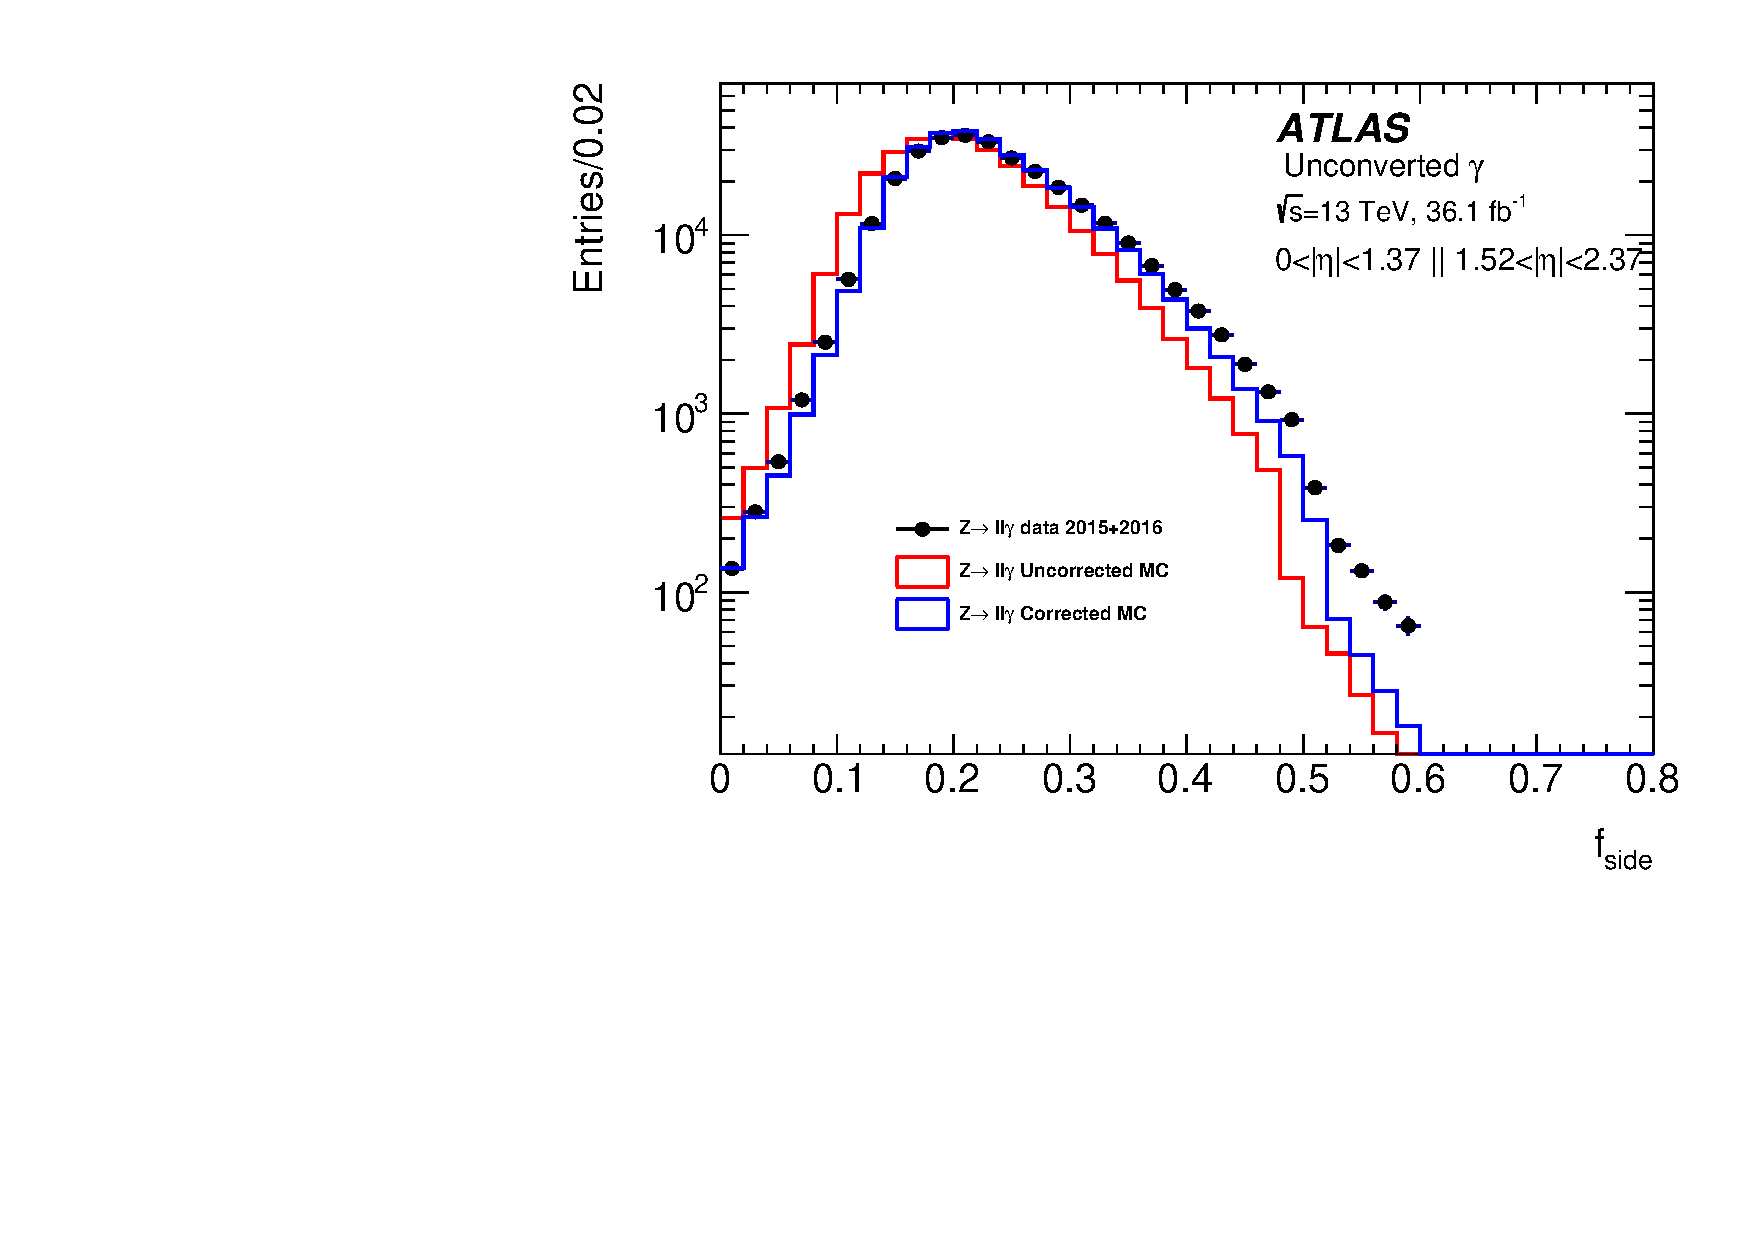
\includegraphics[width=\linewidth]{4_photonid/introduction/shower_shapes/ss_fside_20152016}
        \caption{\fside}
        \label{fig:pid_ss:ss_differences:ss:fside}
    \end{subfigure}
    \hfill
    \begin{subfigure}[h]{0.32\linewidth}
        \centering
        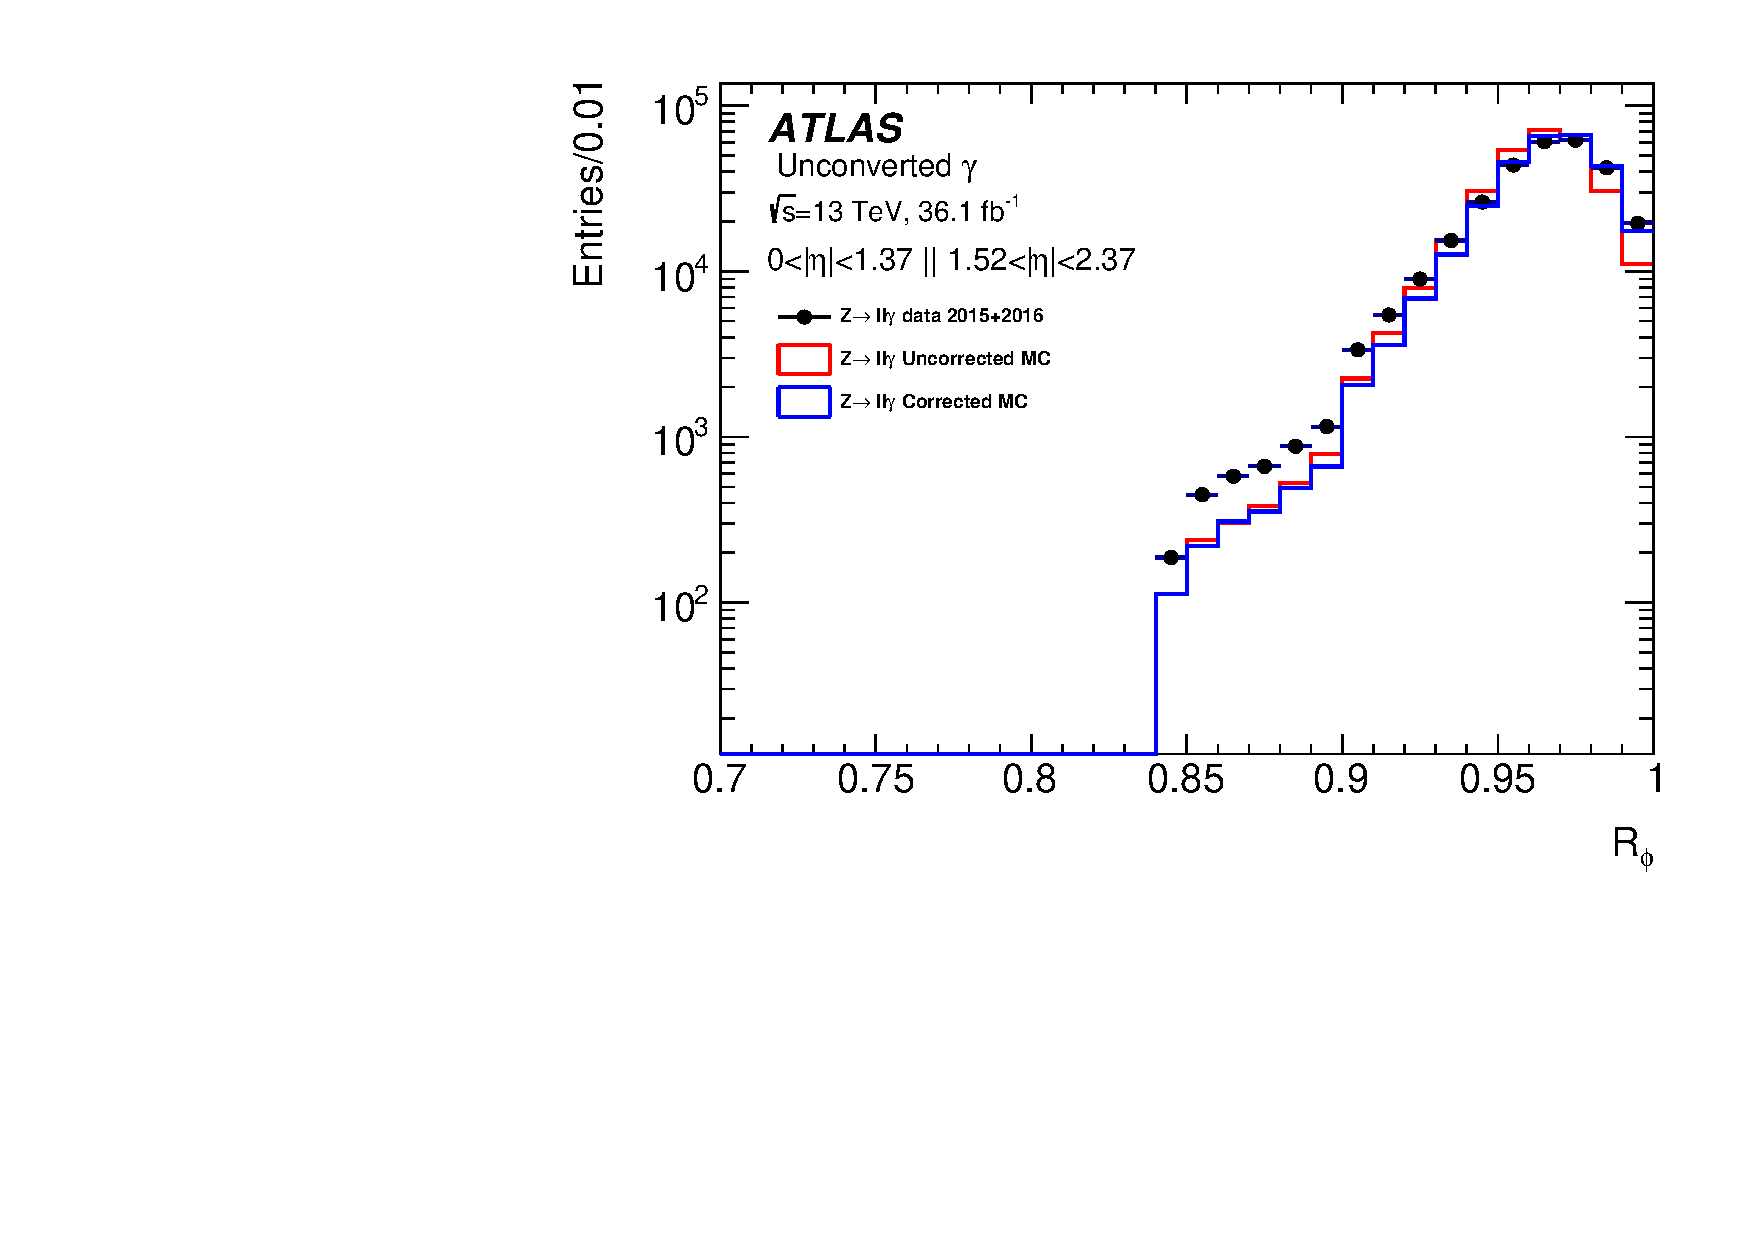
\includegraphics[width=\linewidth]{4_photonid/introduction/shower_shapes/ss_rphi_20152016}
        \caption{\rphi}
        \label{fig:pid_ss:ss_differences:ss:rphi}
    \end{subfigure}
    \hfill
    \begin{subfigure}[h]{0.32\linewidth}
        \centering
        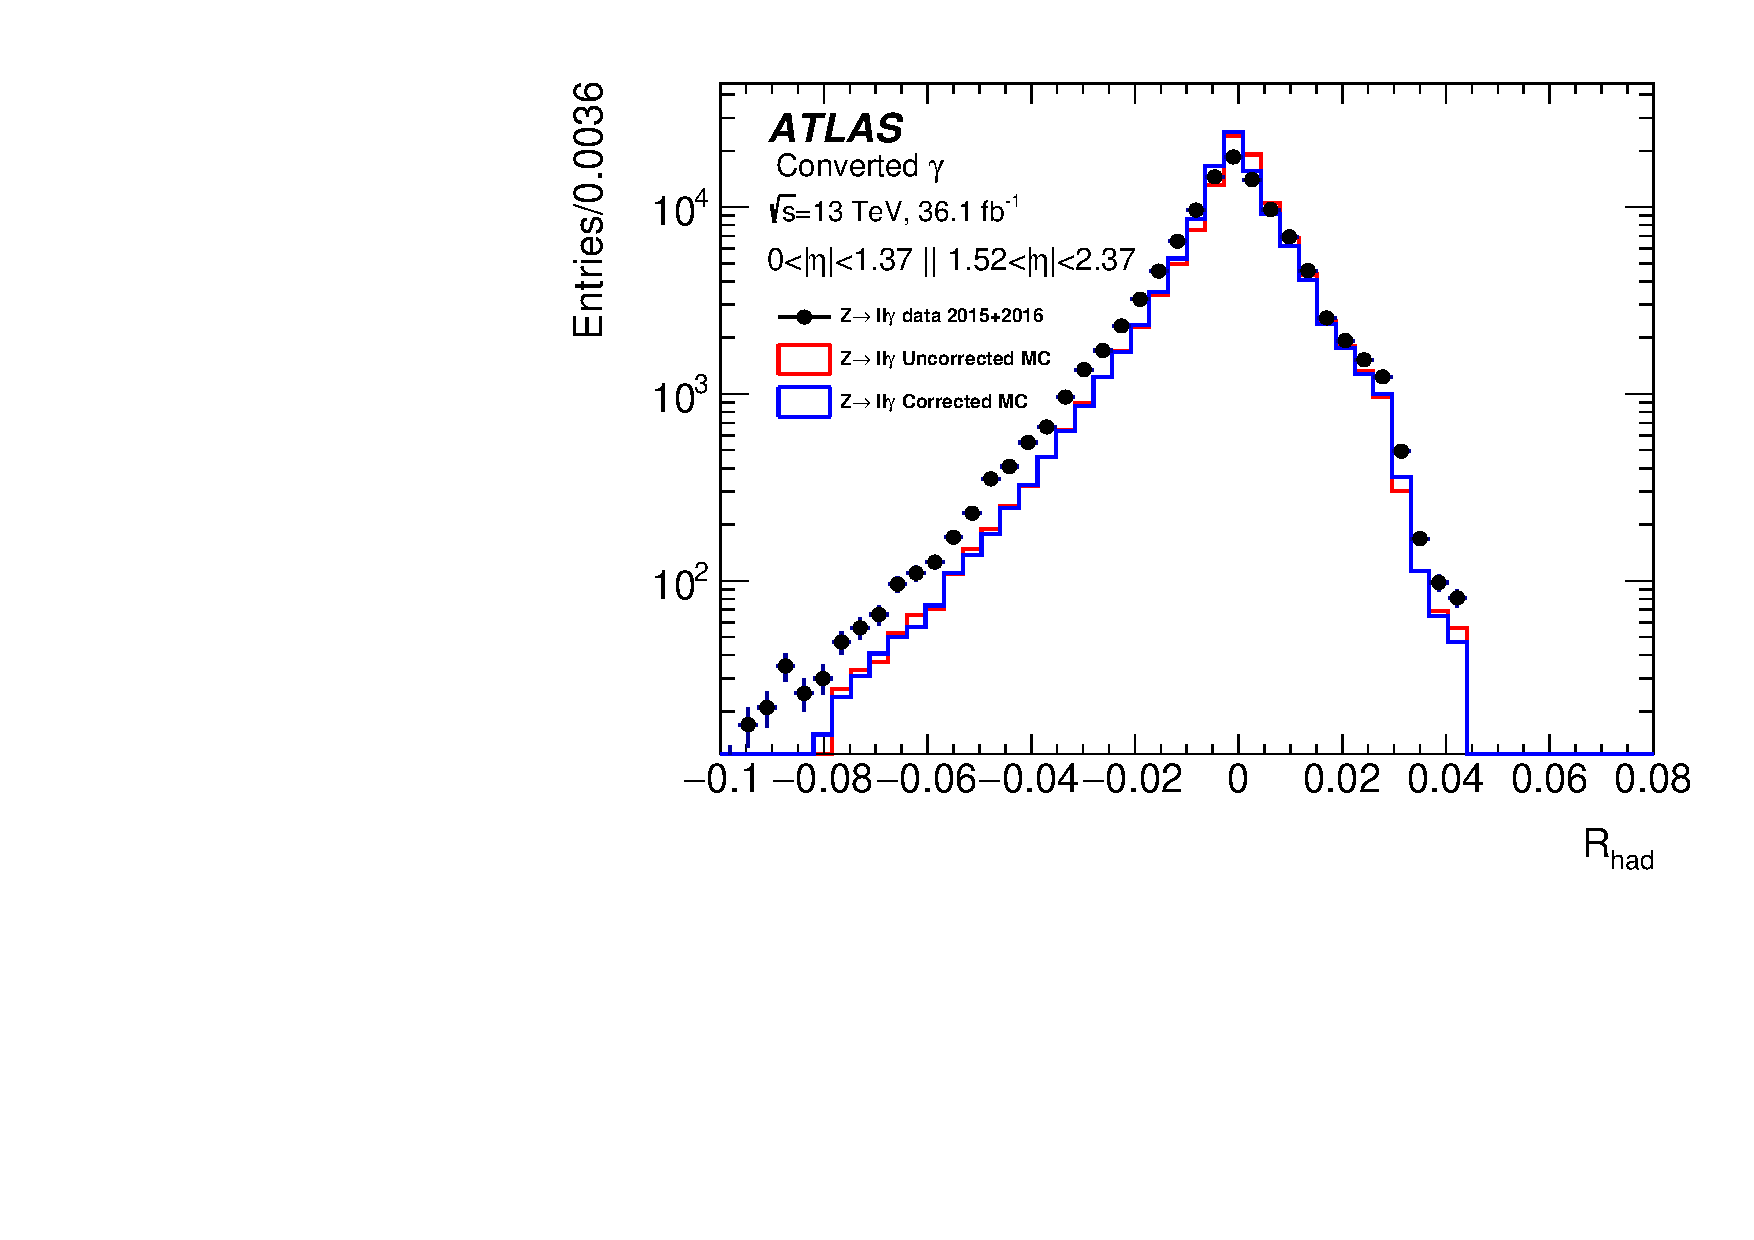
\includegraphics[width=\linewidth]{4_photonid/introduction/shower_shapes/ss_rhad_20152016}
        \caption{\rhad}
        \label{fig:pid_ss:ss_differences:ss:rhad}
    \end{subfigure}
    \caption{Example of \acp{SS} comparisons between data (black dots) against nominal (red line) and corrected (blue line) \ac{MC} simulation, using the full Run-2 \ac{RZ} photon sample~\cite{ATLAS-EGamma-Calibration-2015-2016}.}
    \label{fig:pid_ss:ss_differences:ss}
\end{figure}

To account for the differences in the \acp{SS}, historically, corrections were made in the form of shifts to each one of the \ac{MC} distributions. These shifts comprised the so-called \acfp{FF}, and were determined using a \chisq minimisation on the comparison of data and \ac{MC} \acp{SS}~\cite{ATLAS-EGamma-Performance-2015-2016,ATLAS-EGamma-Performance-2015-2017}.
Even though the mean value differences decreased substantially after these corrections as seen for example in the case of \fside in \Fig{\ref{fig:pid_ss:ss_differences:ss:fside}}, residual but notable differences remained. It is seen from the distributions that the main differences that remained are related to the shape of them, therefore needing for higher order corrections. In the following chapter, a detailed description of newly derived corrections is presented.
Moreover, since \acp{SS} are built from energy deposits on the \ac{ECAL} cells, another possible way of correcting the current disagreement between data and \ac{MC} \acp{SS} is to directly correct the energies on \ac{MC} at a cell-level, fixing the differences in all \acp{SSV} at once. This new approach is described as well in the following chapter.
